\documentclass{beamer}
\usepackage{amsmath,amssymb,latexsym,array,fancyheadings,mathdots}
\usepackage{algorithm,algorithmic}
\usepackage{hyperref}
\usepackage{color}
\usepackage{tabularx}
\usepackage[all]{xy}
\usepackage{qtree}
\usepackage{gitinfo2}

%% RCS
%\usepackage{rcs}

%% Colors
\definecolor{darkgreen}{rgb}{0,.4,0}
\definecolor{darkred}{rgb}{.5,0,0}
\definecolor{darkmagenta}{rgb}{.5,0,.5}
\definecolor{orange}{rgb}{1,.5,0}
\definecolor{lightblue}{rgb}{0.122,0.016,0.855}
\definecolor{darkocre}{rgb}{0.471,0.298,0.008}

\usetheme{default}

%% New Theorems
\newtheorem{thm}{Theorem}
\newtheorem{exm}[thm]{Example}
\newtheorem{cor}[thm]{Corollary}
\newtheorem{propo}[thm]{Proposition}
\newtheorem{lem}[thm]{Lemma}
\newtheorem{clm}[thm]{Claim}
\newtheorem{exr}[thm]{Exercise}
\newtheorem{dfn}[thm]{Definition}

%% New commands
\newcommand{\classfont}{\mathsf}
\newcommand{\ATM}{\classfont{A}_{\mathrm{TM}}}
\newcommand{\MTF}{\mathrm{MTF}}
\newcommand{\OPT}{\mathrm{OPT}}
\newcommand{\ALG}{\mathrm{ALG}}
\newcommand{\ALGNAIVE}{\mathrm{ALG}_{\text{na{\"\i}ve}}}
\newcommand{\LRU}{\mathrm{LRU}}
\newcommand{\FIFO}{\mathrm{FIFO}}
\newcommand{\FWF}{\mathrm{FWF}}
\newcommand{\LFD}{\mathrm{LFD}}
\newcommand{\true}{\mathsf{T}}
\newcommand{\false}{\mathsf{F}}
\newcommand{\also}{\wedge}
\newcommand{\lra}{\leftrightarrow}
\newcommand{\tc}{\textcolor}
\newcommand{\df}[1]{\textcolor{red}{\em #1}}
\newcommand{\highlight}[1]{\textcolor{orange}{\em #1}}
\newcommand{\hl}[1]{\textcolor{blue}{\em #1}}
\newcommand{\amp}{\texttt{\&}}
\newcommand{\hsh}{\texttt{\#}}
\newcommand{\ra}{\rightarrow}
\newcommand{\longra}{\longrightarrow}
\newcommand{\Ra}{\Rightarrow}
\newcommand{\rab}{{\rightarrow_\beta}}
\newcommand{\srab}{{\rightarrow^*_\beta}}
\newcommand{\aeq}{{=_\alpha}}
\newcommand{\order}{\mathrm{order}}
\newcommand{\rem}{\mathrm{rem}}
\newcommand{\IP}{\mathbf{IP}}
\newcommand{\PSPACE}{\mathbf{PSPACE}}
\newcommand{\thevalue}{\text{value}}
\newcommand{\pol}[1]{\mathbf{#1}}
\newcommand{\enc}{\text{Enc}}
\newcommand{\xor}{\oplus}
\newcommand{\zo}{\{0,1\}}
\newcommand{\SOPT}{S_{\mathrm{opt}}}
\newcommand{\la}{\leftarrow}
\newcommand{\myurl}[1]{\textcolor{darkgreen}{\url{#1}}}
\newcommand{\myhref}[2]{\textcolor{darkgreen}{\href{#1}{#2}}}
\newcommand{\qaccept}{q_{\mathrm{accept}}}
\newcommand{\qreject}{q_{\mathrm{reject}}}
\newcommand{\opt}{\text{\sc Opt}}
\newcommand{\tr}{\mathrm{tr}}
\newcommand{\csanky}{p^{\textsc{csanky}}}
\newcommand{\berk}{p^{\textsc{berk}}}

%% Algorithms package customization
\renewcommand{\algorithmicrequire}{\textbf{Pre-condition:}} 
\renewcommand{\algorithmicensure}{\textbf{Post-condition:}} 
\algsetup{indent=3em}

\input{prooftree}

%% including/excluding pauses
\newcommand{\ifpause}{\iftrue} % for including pauses
%\newcommand{\ifpause}{\iffalse} % for excluding pauses

%% 2nd or 3rd edition
\newif\ifthird
\thirdtrue
%\thirdfalse

%disables usefoottemplate
\setbeamertemplate{navigation symbols}{}
%\setbeamertemplate{footline}% 
%{\strut\quad\tiny 
%\begin{minipage}{3cm}
%Cryptography - Michael Soltys
%\today\ {\tt v\RCSRevision}
%\end{minipage}\hfill
%\insertsection\
%- \insertframenumber/\inserttotalframenumber\quad\strut}

\newcommand{\mytitle}{Computational Foundations}
\newcommand{\mychpnr}{9}
%% Title page contents
\title{Intro to Analysis of Algorithms \\ \mytitle \\  Chapter \mychpnr}
\author{Michael Soltys}
\date{\textcolor{darkgreen}{\tiny\tt 
[ {\bf Git} Date:\gitAuthorDate\ 
Hash:\gitAbbrevHash\ 
Ed:\ifthird
3rd
\else
2nd
\fi]}}
\institute{CSU Channel Islands}

\setbeamertemplate{footline}{
  \colorbox{white}{\color{black}\tt
     \begin{tabularx}{0.97\textwidth}{XXX}
          IAA Chp \mychpnr\ - Michael Soltys \copyright & 
          \hfill\today\ (\gitAbbrevHash; \ifthird ed3\else ed2\fi)
					\hfill\phantom{.} & 
          \hfill\insertsection\ - \insertframenumber/\inserttotalframenumber \\
      \end{tabularx}}}

\begin{document}

\mode<presentation>
{
}

\parskip 8pt

\section{Introduction}

\begin{frame}
\titlepage
\end{frame}


\section{Introduction}

\begin{frame}
\begin{center}
{\bf Outline}
\end{center}

\begin{center}
\begin{minipage}{6cm}
\begin{tabbing}
\= Alphabets, strings and languages \\
\> Regular languages \\
\> Context-free languages \\
\> Turing machines \\
\> $\lambda$-calculus (not in textbook) \\ 
\> Recursive functions (not in textbook) \\ 
\> Conclusion
\end{tabbing}
\end{minipage}
\end{center}
\end{frame}

\section{Basics}

\begin{frame}
\begin{center}
\addtocounter{part}{1}
{\bf Sections 9.1 \&\ 9.2: \\ Alphabets, strings and languages}
\end{center}
\end{frame}

\begin{frame}
Since long ago ``markings'' have been used to store \&\ process information.
The following pictures are from the {\em Smithsonian Museum of Natural
History, Washington D.C.}
\begin{tabbing}
\begin{minipage}{6cm}
\raggedright
{\bf Engraved ocher plaque} \\
Blombos Cave, South Africa \\
77,000--75,000 years old
\end{minipage}
\=\begin{minipage}{6cm}
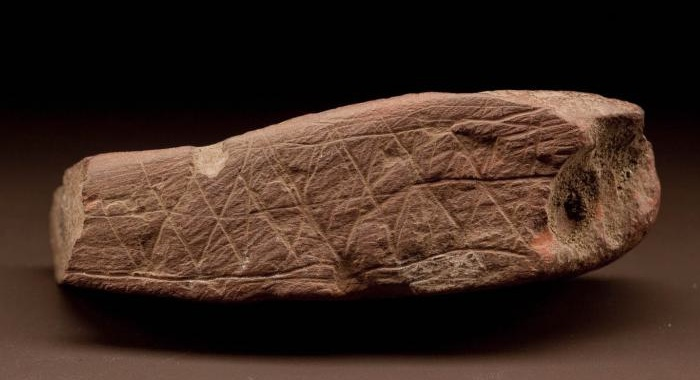
\includegraphics[width=2cm]{figures/ocher.jpg}
\hskip 2mm
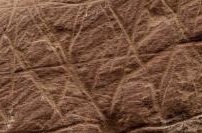
\includegraphics[width=3cm]{figures/ocher-zoom.jpg}
\end{minipage} \\[2mm]
\begin{minipage}{6cm}
\raggedright
{\bf Ishango bone} \\
Congo, 25,000--20,000 years old \\
leg bone from a baboon; 3~rows of tally marks,
to {\em add} or {\em multiply} ({\bf ?})
\end{minipage}
\>\begin{minipage}{5cm}
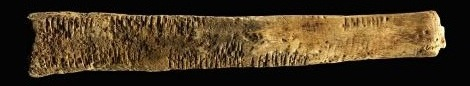
\includegraphics[width=5cm]{figures/ishango.jpg}
\end{minipage} \\[2mm]
\begin{minipage}{6cm}
\raggedright
{\bf Reindeer antler with tally marks} \\
La Madeleine, France \\
17,000--11,500 years old
\end{minipage}
\>\begin{minipage}{5cm}
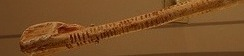
\includegraphics[width=5cm]{figures/antler.jpg}
\end{minipage}
\end{tabbing}
\end{frame}

\begin{frame}

About 8,000 years ago, humans were using symbols to represent words
and concepts.
True forms of writing developed over the next few thousand years. 

\begin{minipage}{5cm}
\raggedright
{\bf Cylinder seals} were rolled accross wet clay tablets to
produce raised designs \\[3mm]
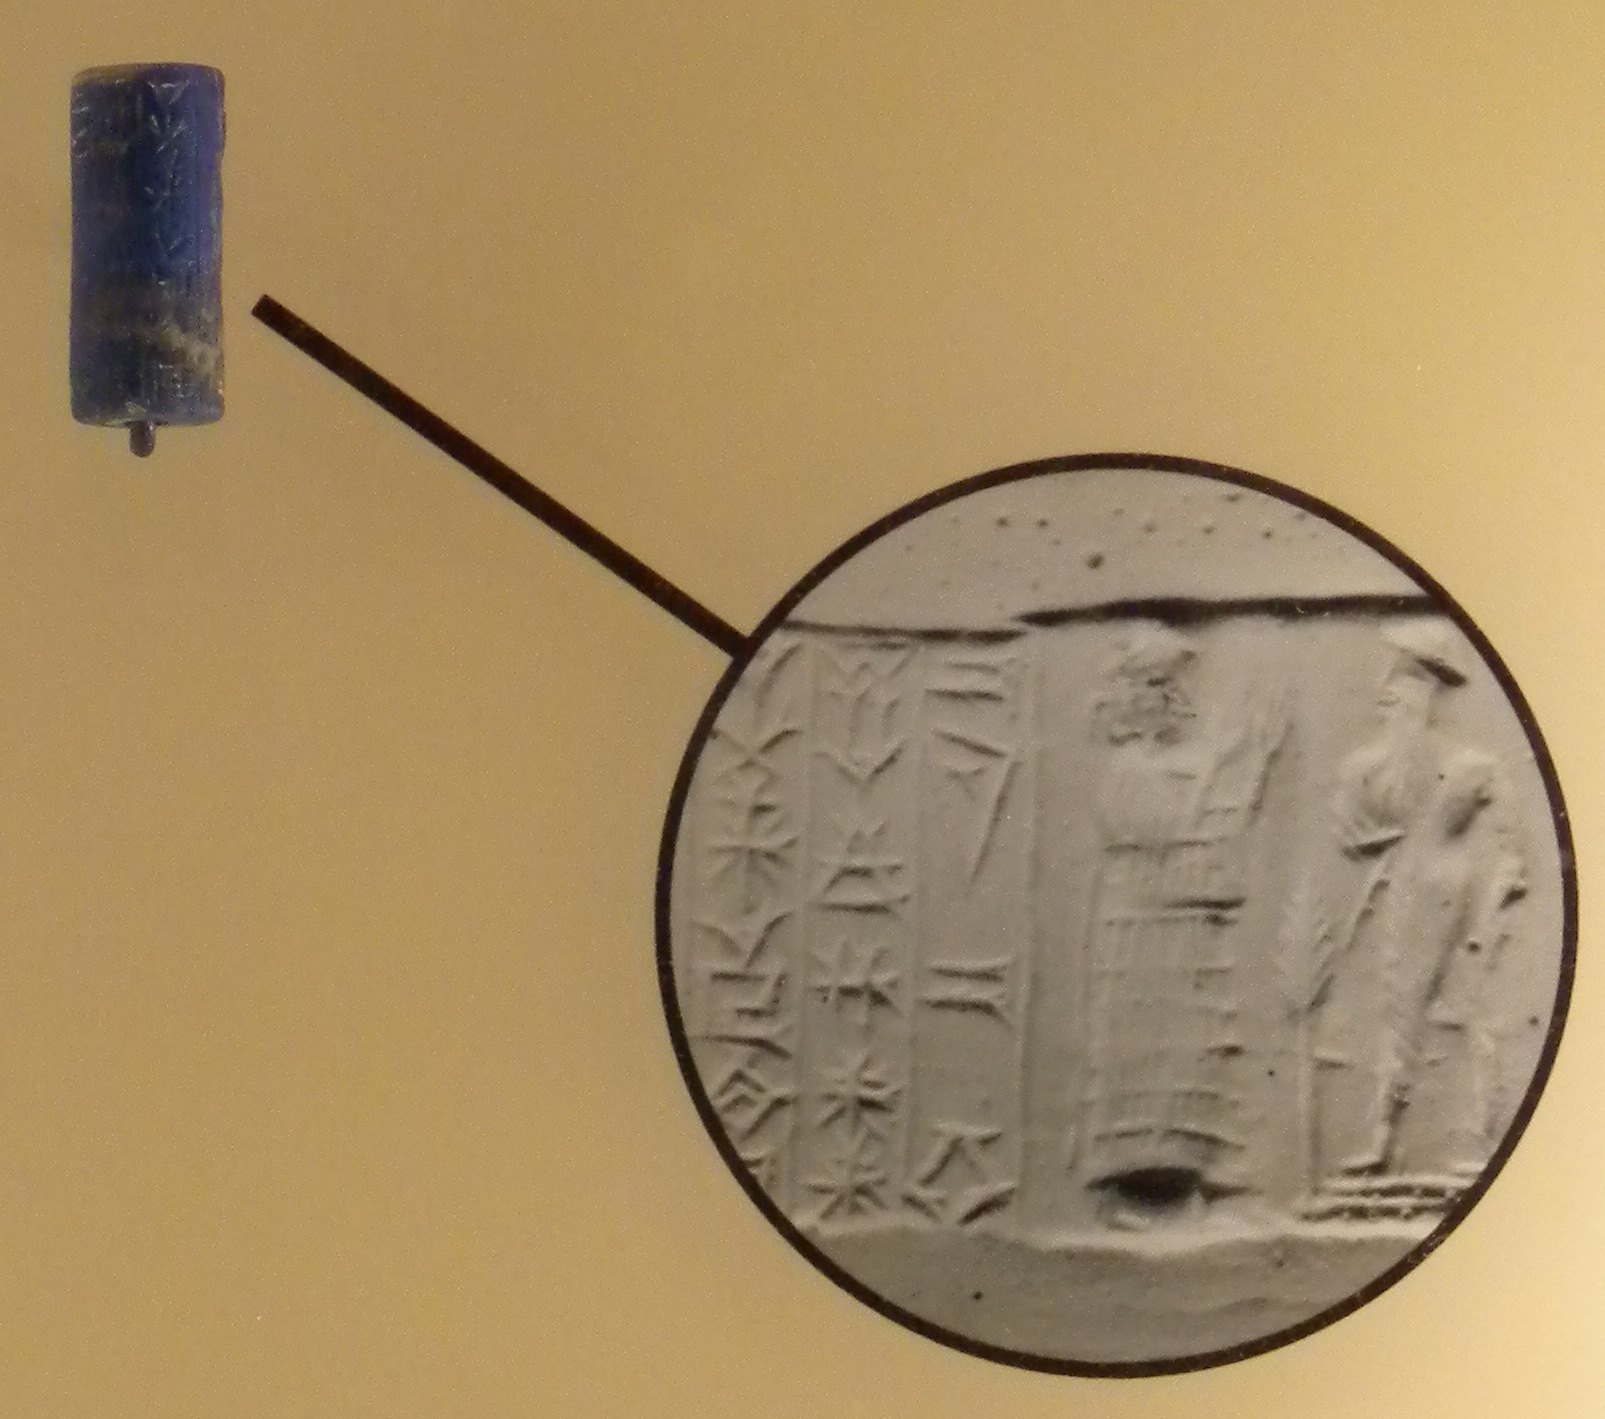
\includegraphics[width=4cm]{figures/cylinder.jpg} \\
cylinder seal in lapis lazuli,
Assyrian culture,
Babylon, Iraq,
4,100--3,600 years ago
\end{minipage}
\begin{minipage}{5.5cm}
\raggedright
{\bf Cuneiform symbols} stood for concepts and later for sounds and
syllables \\[3mm]
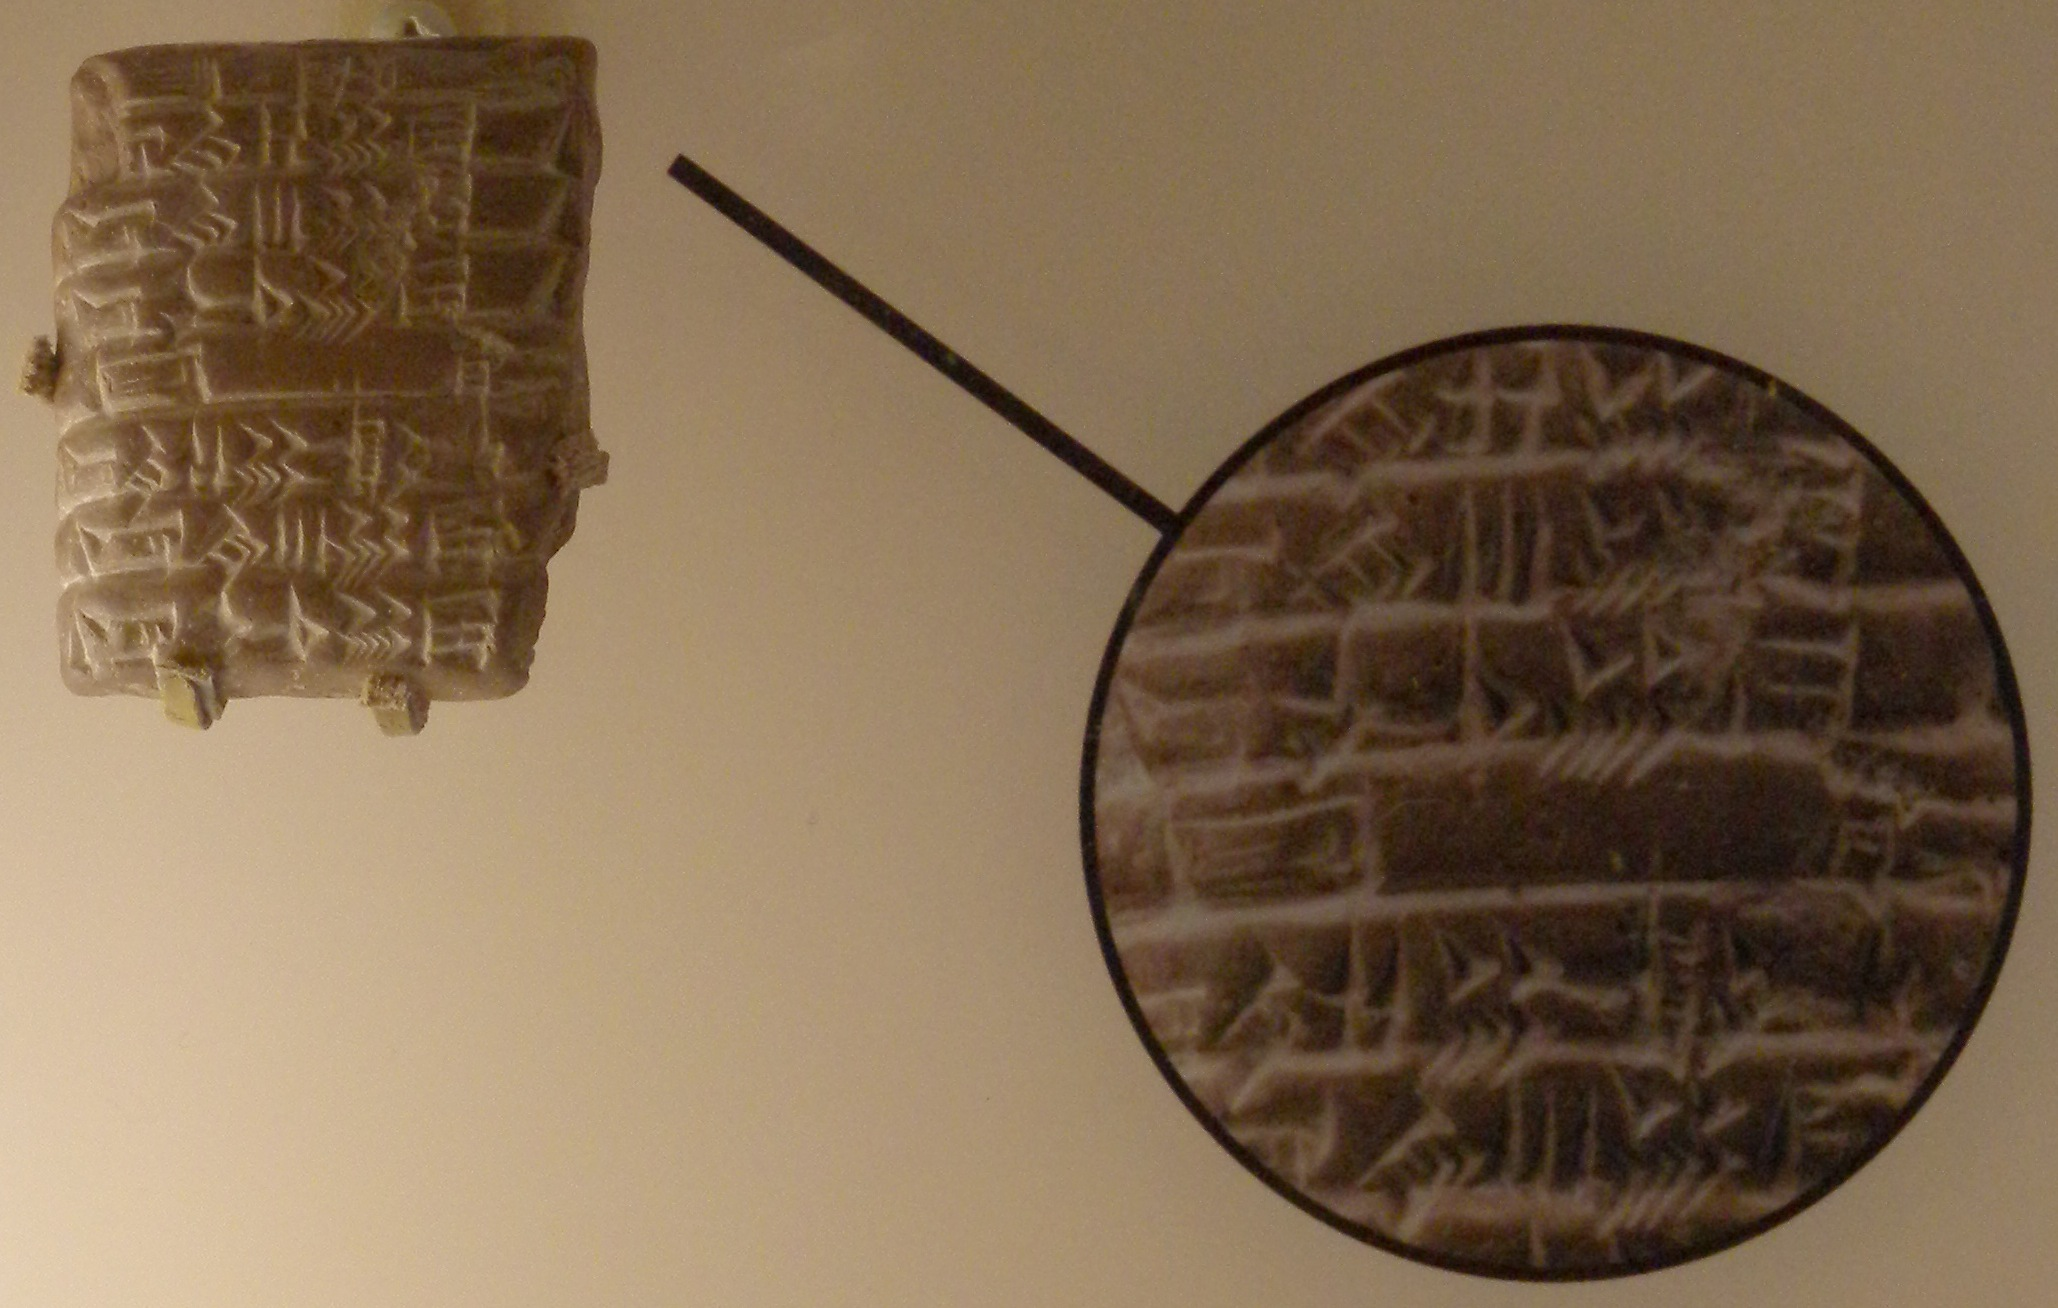
\includegraphics[width=5.5cm]{figures/cuneiform.jpg} \\
cuneiform clay tablet,
Chakma, Chalush, near Babylon, Iraq,
4,000--2,600 years ago
\end{minipage}
\end{frame}

\begin{frame}

\begin{center}
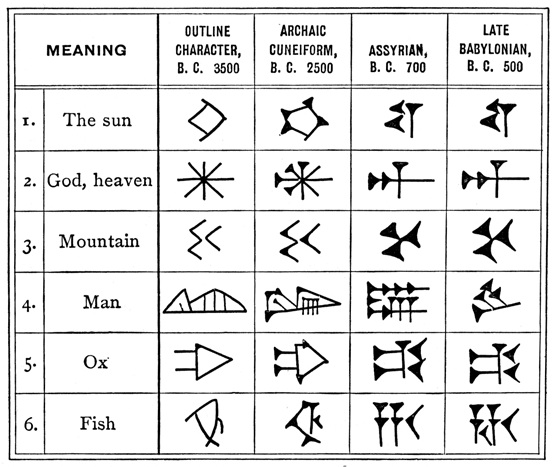
\includegraphics[width=8cm]{figures/cuneiform-symbols.jpg}
\end{center}
\end{frame}

\begin{frame}
An \df{alphabet} is a finite, non-empty set of
distinct symbols, denoted usually by $\Sigma$.

e.g., $\Sigma=\{0,1\}$ (binary alphabet) \\
$\Sigma=\{a,b,c,\ldots,z\}$ (lower-case letters alphabet)

A \df{string}, also called \df{word}, is a finite
ordered sequence of symbols chosen from some alphabet.

e.g., 010011101011

$|w|$ denotes the \df{length} of the string $w$.

e.g., $|010011101011|=12$

The \df{empty string}, $\varepsilon$,
$|\varepsilon|=0$, is in any $\Sigma$ by default.
\end{frame}

\begin{frame}
$\Sigma^k$ is the set of strings over $\Sigma$ of length {\em exactly}
$k$.  

e.g., If $\Sigma=\{0,1\}$, then 
\begin{align*}
\Sigma^0 &=\{\varepsilon\} \\
\Sigma^1 &=\Sigma \\
\Sigma^2 &=\{00,01,10,11\}, \text{ etc. } 
|\Sigma^k|?
\end{align*}

\df{Kleene's star}  $\Sigma^*$ is the set of all strings over
$\Sigma$.  

$\Sigma^*=\Sigma^0\cup
\underbrace{\Sigma^1\cup\Sigma^2\cup\Sigma^3\cup\ldots}_{=\Sigma^+}$

\df{Concatenation}  If $x,y$ are strings, and
$x=a_1a_2\ldots a_m$ \amp\ $y=b_1b_2\ldots b_n \Rightarrow$
$x\cdot y=\underbrace{xy}_{\text{\df{juxtaposition}}}
=a_1a_2\ldots a_mb_1b_2\ldots b_n$
\end{frame}

\begin{frame}
\begin{minipage}{5cm}
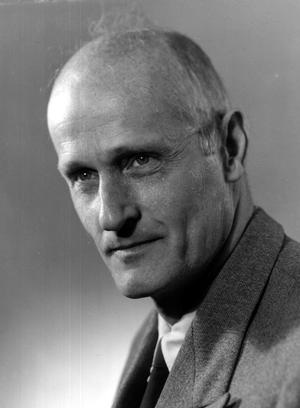
\includegraphics[width=4cm]{figures/StephenKleene.jpg}
\end{minipage}
\begin{minipage}{5cm}
\myhref{http://en.wikipedia.org/wiki/Stephen_Cole_Kleene}{Stephen Cole Kleene} \\
\end{minipage}
\end{frame}

\begin{frame}
A \df{language} $L$ is a collection of strings over some
alphabet $\Sigma$, i.e.,  $L\subseteq\Sigma^*$. E.g.,
\begin{equation}\label{eq:example}
L=\{\varepsilon,01,0011,000111,\ldots\}=\{0^n1^n|n\ge 0\}
\end{equation}

Note:

\begin{itemize}
\item  $w\varepsilon=\varepsilon w=w$.

\item $\{\varepsilon\}\neq\emptyset$; one is the language
consisting of the single string $\varepsilon$, and the other is the
empty language.

\end{itemize}
\end{frame}

\begin{frame}
Two fundamental questions:
\begin{itemize}
\item  How do we describe a language?  (\ref{eq:example}) is just an
{\em informal set-theoretic} description.

\item  Given a language $L\subseteq\Sigma^*$ and a string
$x\in\Sigma^*$, how do we check if $x\in L$?  E.g.,

$$
L=\{\underbrace{10}_2,\underbrace{11}_3,\underbrace{101}_5,
\underbrace{111}_7,\ldots\}\subseteq\{0,1\}^*
$$

$w\in L$ iff $w\in\{0,1\}^*$ encodes a prime number in standard binary
notation.

\item What is an algorithm?
\end{itemize}
\end{frame}

\section{DFAs}

\begin{frame}
\begin{center}
\addtocounter{part}{1}
{\bf Section 9.3: \\ Regular languages}
\end{center}
\end{frame}

\begin{frame}
\df{Deterministic Finite Automaton (DFA)}  

$A=(Q,\Sigma,\delta,q_0,F)$

\begin{itemize}
\item  Finite set of states $Q$
\item  Finite set of input symbols $\Sigma$
\item  Transition fn $\delta:Q\times\Sigma\longrightarrow Q$;
given $q\in Q,a\in\Sigma$, $\delta(q,a)=p\in Q$ 
\item  Start state $q_0$
\item  A set of final (accepting) states.
\end{itemize}

To see whether $A$ accepts a string
$w$, we ``run'' $A$ on $w=a_1a_2\ldots a_n$ as follows:

$\delta(q_0,a_1)=q_1$, $\delta(q_1,a_2)=q_2$, until
$\delta(q_{n-1},a_n)=q_n$.  

Accept iff $q_n\in F$.
\end{frame}

\begin{frame}
\begin{minipage}{5cm}
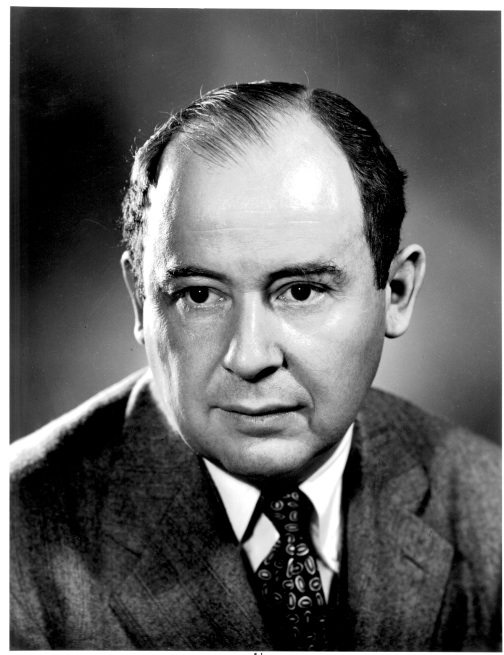
\includegraphics[width=4cm]{figures/JohnvonNeumann.jpg}
\end{minipage}
\begin{minipage}{5cm}
\myhref{http://en.wikipedia.org/wiki/John_von_Neumann}{John von Neumann} \\
\end{minipage}
\end{frame}

\begin{frame}
Consider $L=\{w|\text{ $w$ is of the form $x01y\in\Sigma^*$ }\}$ where
$\Sigma=\{0,1\}$.

We want to specify a DFA $A=(Q,\Sigma,\delta,q_0,F)$ that accepts all
and only the strings in $L$.

$\Sigma=\{0,1\}$, $Q=\{q_0,q_1,q_2\}$, and $F=\{q_1\}$.

\df{Transition diagram}
\begin{tabular}{l}
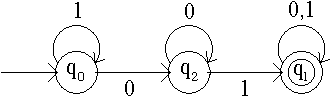
\includegraphics{figures/1.pdf}
\end{tabular}

\df{Transition table}
\begin{tabular}{c||c|c}
       & $0$   & $1$   \\\hline\hline
$q_0$  & $q_2$ & $q_0$ \\\hline
$q_1$  & $q_1$ & $q_1$ \\\hline
$q_2$  & $q_2$ & $q_1$
\end{tabular}
\end{frame}

\begin{frame}
\df{Extended Transition Function (ETF)}  given $\delta$, its ETF is
$\hat\delta$ defined inductively:

Basis Case: $\hat\delta(q,\varepsilon)=q$

Induction Step: if $w=xa$, $w,x\in\Sigma^*$ and $a\in\Sigma$, then
$$
\hat\delta(q,w)=\hat\delta(q,xa)=\delta(\hat\delta(q,x),a)
$$ 
Thus: $\hat\delta:Q\times\Sigma^*\longrightarrow Q$.

$w\in L(A) \iff \hat\delta(q_0,w)\in F$

Here $L(A)$ is the set of all those strings (and only those) which are
accepted by $A$.
\end{frame}

\begin{frame}
\df{Language of a DFA:} $L(A)=\{w|\hat\delta(q_0,w)\in F\}$

Note that
\begin{itemize}
\item $A$ is a {\em syntactic} object
\item while $L(A)$ is a {\em semantic} object
\end{itemize}
Thus $L$ is a function that assigns a {\em meaning} or {\em
interpretation} to a syntactic object.

\df{Regular Languages:} $L$ is {\em regular} iff there exists a DFA
$A$ such that $L=L(A)$.
\end{frame}

\begin{frame}
\df{Nondeterministic Finite Automata (NFA)}

The transition function $\delta$ becomes a transition relation,
i.e., $\delta\subseteq Q\times\Sigma\times Q$, i.e., on the
same pair $(q,a)$ there may be more than one possible new state (or
none).

Equivalently, we can look at $\delta$ as
$\delta:Q\times\Sigma\longrightarrow\mathcal{P}(Q)$, where
$\mathcal{P}(Q)$ is the power set of $Q$.

$L_n=\{w|\text{ $n$-th symbol from the end is 1 }\}$ \\
What is an NFA for $L_n$
\begin{center}
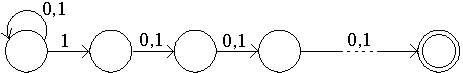
\includegraphics[width=7cm]{figures/2.pdf}
\end{center}
At least how many states does any DFA recognizing $L_n$ require?
\end{frame}

\begin{frame}
NFA with $\varepsilon$ transitions: $\varepsilon$-NFA:
$\delta:Q\times(\Sigma\cup\{\varepsilon\})\longrightarrow\mathcal{P}(Q)$

\begin{center}
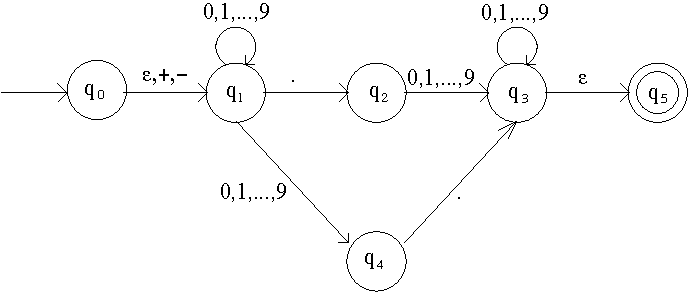
\includegraphics[width=8cm]{figures/3.pdf}
\end{center}
\end{frame}

\begin{frame}
To define $\hat\delta$ for $\varepsilon$-NFAs we need the concept of
$\varepsilon$-closure.

Given $q$, $\varepsilon$-close$(q)$ is the set of all states $p$ which
are reachable from $q$ by following arrows labeled by $\varepsilon$.

Formally, $q\in\varepsilon\text{-close}(q)$, and if
$p\in\varepsilon\text{-close}(q)$, and
$p\stackrel{\varepsilon}{\longrightarrow}r$, then
$r\in\varepsilon\text{-close}(q)$.

$\hat\delta(q,\varepsilon)=\varepsilon\text{-close}(q)$

Suppose $w=xa$, $\hat\delta(q,x)=\{p_1,p_2,\ldots,p_n\}$, \\
and $\cup_{i=1}^n\delta(p_i,a)=\{r_1,r_2,\ldots,r_m\}$, \\
then
$$
\hat\delta(q,w)=\cup_{i=1}^m\varepsilon\text{-close}(r_i)
$$
\end{frame}

\begin{frame}

{\bf Theorem:}  DFAs and $\varepsilon$-NFAs are equivalent.

{\bf Proof:}  Slightly modified subset construction.

$q^D_0=\varepsilon\text{-close}(\{q^N_0\})$

$\delta_D(R,a)=\cup_{r\in R}\varepsilon\text{-close}(\delta_N(r,a))$

Given a set of states $S$, its $\varepsilon$-closure is the union of
the $\varepsilon$-closures of its members.  

The states of $D$ are those subsets $S\subseteq Q_N$ which are equal
to their $\varepsilon$-closures. 

{\bf Corollary:}
A language is regular \\
$\iff$ it is recognized by some DFA \\
$\iff$ it is recognized by some NFA \\
$\iff$ it is recognized by some $\varepsilon$-NFA
\end{frame}

\begin{frame}

Union: $L\cup M=\{w|w\in L\text{ or }w\in M\}$ \\
Concatenation: $LM=\{xy|x\in L\text{ and }y\in M\}$ \\
Star (or closure): $L^*=\{w|w=x_1x_2\ldots x_n\text{ and }x_i\in L\}$

\df{Regular Expressions}

Basis Case: $a\in\Sigma,\varepsilon,\emptyset$

Induction Step: If $E,F$ are regular expressions, the so are
$E+F,EF,(E)^*,(E)$.

What are $L(a),L(\varepsilon),L(\emptyset),L(E+F),L(EF),L(E^*)$?

%Sipser 3.1.3(a)
Ex. Give a reg exp for the set of strings of 0s and 1s not
containing 101 as a substring:
$$
(\varepsilon+0)(1^*+00^*0)^*(\varepsilon+0)
$$
\end{frame}

\begin{frame}

{\bf Theorem:}  A language is regular iff it is given by some regular
expression.

{\bf Proof:}  reg exp $\Longrightarrow$ $\varepsilon$-NFA \&\
DFA $\Longrightarrow$ reg exp

$[\Longrightarrow]$

Use structural induction to convert $R$ to an $\varepsilon$-NFA with
3 properties:
\begin{enumerate}
\item  Exactly one accepting state
\item  No arrow into the initial state
\item  No arrow out of the accepting state
\end{enumerate}

Basis Case: $\varepsilon,\emptyset,a\in\Sigma$

\begin{center}
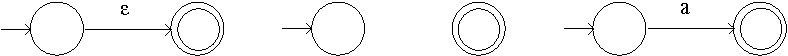
\includegraphics[width=10cm]{figures/4.pdf}
\end{center}
\end{frame}

\begin{frame}
Induction Step: $R+S,RS,R^*,(R)$

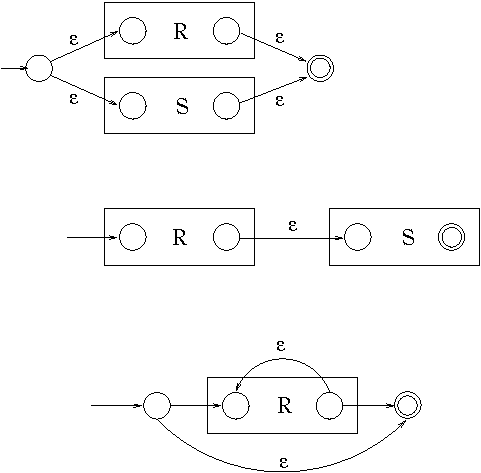
\includegraphics[height=6cm]{figures/5.pdf}
\end{frame}

\begin{frame}
$[\Longleftarrow]$ Convert DFA to reg exp.

{\bf Method 1}

Suppose $A$ has $n$ states.  $R^{(k)}_{ij}$ denotes the reg exp whose
language is the set of strings $w$ such that:
\begin{quote}
$w$ takes $A$ from state $i$ to state $j$ with all intermediate states
$\le k$
\end{quote}
What is $R$ such that $L(R)=L(A)$?

$R=R_{1j_1}^{(n)}+R_{1j_2}^{(n)}+\cdots+R_{1j_k}^{(n)}$
where $F=\{j_1,j_2,\ldots,j_k\}$

Build $R_{ij}^{(k)}$ by induction on $k$.

Basis Case: $k=0$, $R_{ij}^{(0)}=x+a_1+a_2+\cdots+a_k$ where
$i\stackrel{a_l}{\longrightarrow}j$ and $x=\emptyset$ if $i\neq j$ and
$x=\varepsilon$ if $i=j$
\end{frame}

\begin{frame}
Induction Step: $k>0$ 
$$
R_{ij}^{(k)}=\underbrace{R_{ij}^{(k-1)}}_{\text{path does not visit $k$}}
+\qquad
\underbrace{R_{ik}^{(k-1)}\left(R_{kk}^{(k-1)}\right)^*
R_{kj}^{(k-1)}}_{\text{visits $k$ at least once}}
$$

{\bf Method 2:}
DFA $\Longrightarrow$ G$\varepsilon$-NFA $\Longrightarrow$ Reg Exp

{\bf Generalized $\varepsilon$-NFA:} 
$$
\delta:(Q-\{q_{\text{accept}}\})\times
(Q-\{q_{\text{start}}\})\longrightarrow\mathcal{R}
$$
where the start and accept states are unique.  

$G$ accepts $w=w_1w_2\ldots w_n$, \underline{$w_i\in\Sigma^*$}, if
there exists a sequence of states
$$
q_0=q_{\text{start}},q_1,\ldots,q_n=q_{\text{accept}}
$$ 
such that for all $i$, $w_i\in L(R_i)$ where
$R_i=\delta(q_{i-1},q_i)$.
\end{frame}

\begin{frame}
When translating from DFA to G$\varepsilon$-NFA, if there is no arrow
$i\longrightarrow j$, we label it with $\emptyset$.  

For each $i$, we label the self-loop with $\varepsilon$.

Eliminate states from $G$ until left with just
$q_{\text{start}}\stackrel{R}{\longrightarrow}q_{\text{accept}}$:

\begin{center}
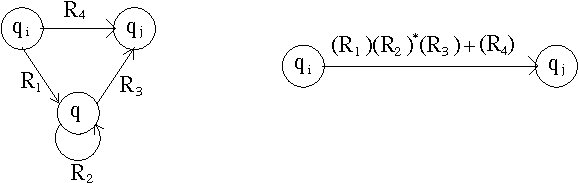
\includegraphics{figures/6.pdf}
\end{center}
\end{frame}

\begin{frame}

{\bf Algebraic Laws for Reg Exps}

$L+M=M+L$ (commutativity of $+$)\\
$(L+M)+N=L+(M+N)$ (associativity of $+$)\\
$(LM)N=L(MN)$ (associativity of concatenation) \\
$LM=ML$ ?

\bigskip

$\emptyset+L=L+\emptyset=L$ ($\emptyset$ identity for $+$) \\
$\varepsilon L=L\varepsilon=L$ ($\varepsilon$ identity for
concatenation) \\
$\emptyset L=L\emptyset =\emptyset$ ($\emptyset$ annihilator for
concatenation)

\bigskip

$L(M+N)=LM+LN$ (left-distributivity) \\
$(M+N)L=ML+NL$ (right-distributivity)
\end{frame}

\begin{frame}
$L+L=L$ (idempotent law for union) \\

\bigskip

Laws with closure:

$(L^*)^*=L^*$ \\
$\emptyset^*=\varepsilon$ \\
$\varepsilon^*=\varepsilon$ \\
$L^+=LL^*=L^*L$ \\
$L^*=L^++\varepsilon$

{\bf Test for Reg Exp Algebraic Law:}

To test whether $E=F$, where $E,F$ are reg exp with variables
($L,M,N,\ldots$), convert $E,F$ to concrete reg exp $C,D$ by
replacing variables by symbols.  If $L(C)=L(D)$, then $E=F$.

Ex. To show $(L+M)^*=(L^*M^*)^*$ replace $L,M$ by $a,b$, to obtain
$(a+b)^*=(a^*b^*)^*$.
\end{frame}

\section{Pumping Lemma}

\begin{frame}

{\bf Pumping Lemma:}  Let $L$ be a regular language.  Then there
exists a constant $n$ (depending on $L$) such that for all $w\in L$,
$|w|\geq n$, we can break $w$ into three parts $w=xyz$ such that:
\begin{enumerate}
\item  $y\neq\varepsilon$
\item  $|xy|\le n$
\item  For all $k\geq 0$, $xy^kz\in L$
\end{enumerate}

Proof:  Suppose $L$ is regular.  Then there exists a DFA $A$ such that
$L=L(A)$.  Let $n$ be the number of states of $A$.   Consider any
$w=a_1a_2\ldots a_m$, $m\geq n$:
$$
{}_{\displaystyle\stackrel{\uparrow}{p_0}}\overbrace{a_1
{}_{\displaystyle\stackrel{\uparrow}{p_1}}a_2
{}_{\displaystyle\stackrel{\uparrow}{p_2}}a_3
\ldots
a_i}^{x}
{}_{\displaystyle\stackrel{\uparrow}{p_i}}\overbrace{a_{i+1}
\ldots
a_j}^{y}
{}_{\displaystyle\stackrel{\uparrow}{p_j}}\overbrace{a_{j+1}
\ldots
a_m}^{z}{}_{\displaystyle\stackrel{\uparrow}{p_{m}}}
$$
\end{frame}

\begin{frame}
Ex. Show $L=\{0^n1^n|n\ge 0\}$ is {\em not} regular.

Suppose it is.  By PL $\exists p$.  Consider $s=0^p1^p=xyz$.  Since
$|xy|\le p$, $y\neq\varepsilon$, $y=0^j$, $j>0$.  And
$xy^2z=0^{p+j}1^p\in L$, which is a contradiction.

Ex. Show $L=\{1^p|\text{ $p$ is prime }\}$ is not regular.

Suppose it is.  By PL $\exists n$.  Consider some prime $p\geq n+2$. 

Let $1^p=xyz$, $|y|=m>0$.  So $|xz|=p-m$.

Consider $xy^{(p-m)}z$ which must be in $L$.  

But $|xy^{(p-m)}z|=|xz|+|y|(p-m)=(p-m)+m(p-m)=(p-m)(1+m)$

Now $1+m>1$ since $y\neq\varepsilon$, and $p-m>1$ since $p>n+2$ and
$m=|y|\le|xy|\le n$.  
So the length of $xy^{(p-m)}z$ is not prime, and
hence it cannot be in $L$ --- contradiction.
\end{frame}

\section{Myhill-Nerode Theorem}

\begin{frame}
$R$ is a \df{relation} on two sets $A,B$ if
$R\subseteq A\times B$.

e.g. $R=\{(m,n)|\text{ $m-n$ is even
}\}\subseteq\mathbb{Z}\times\mathbb{Z}$. \\
So $(3,5),(2,-4)\in R$, but $(-2,1)\notin R$.

$R$ is an \df{equivalence relation} if it is
\begin{enumerate}
\item  Reflexive: for all $a$, $(a,a)\in R$
\item  Symmetric: for all $a,b$, $(a,b)\in R\Rightarrow(b,a)\in R$
\item  Transitive: for all $a,b,c$, $(a,b)\in R$ and $(b,c)\in R$,
implies that $(a,c)\in R$.
\end{enumerate}
If $R$ is an equivalence relation, and $(a,b)\in R$, then we write
$a\equiv_R b$ or just $a\equiv b$.

Equivalence class: $[a]=\{x|x\equiv a\}$
\end{frame}

\begin{frame}

{\bf Theorem:}  For any equivalence relation:
\begin{enumerate}
\item  $a\in[a]$
\item  $a\equiv b\iff [a]=[b]$
\item  $a\not\equiv b$ then $[a]\cap[b]=\emptyset$
\item  any two equivalence classes are either equal or disjoint.
\end{enumerate}

{\bf Proof:}  3. prove the contra-positive: suppose
$[a]\cap[b]\neq\emptyset$, so there exists an $x\in[a]\cap[b]$.  

By definition, $x\equiv a$ and $x\equiv b$.  

By symmetry and transitivity, $a\equiv b$.
\end{frame}

\begin{frame}

$L\subseteq\Sigma^*$;
given $x,y\in\Sigma^*$ we say that they are \df{distinguishable} if
$\exists z\in\Sigma^*$ such that exactly one of $xz,yz$ is in $L$.

E.g., $L=\{w\in\{0,1\}^*|\text{ $w$ has an even number of 1s }\}$, and
$x=00,y=10$.  Then $x,y$ are distinguishable because letting $z=1$,
$xz=001\not\in L$ but $yz=101\in L$.

Given $L$, let $\equiv_L$ be the relation: $x\equiv_Ly$ iff $x,y$ are
{\em not} distinguishable.  Then $\equiv_L$ is an equivalence
relation.

{\bf Myhill-Nerode Theorem:}  $L$ is regular $\iff$ $\equiv_L$ has
{\em finitely many} equivalence classes.

Moreover, the number of states in the smallest
DFA recognizing $L$ is equal to the number of
equivalence classes of $\equiv_L$.
\end{frame}

\begin{frame}

{\bf Closure Properties of Regular Languages}

{\bf Union:} If $L,M$ are regular, so is $L\cup M$.

Proof: $L=L(R)$ and $M=L(S)$, so $L\cup M=L(R+S)$.

{\bf Complementation:} If $L$ is regular, so is $L^c=\Sigma^*-L$.

Proof: $L=L(A)$, so $L^c=L(A')$, where $A'$ is the DFA obtained from
$A$ as follows: $F_{A'}=Q-F_A$.

{\bf Intersection:} If $L,M$ are regular, so is $L\cap M$.

Proof: $L\cap M=\overline{\overline{L}\cup\overline{M}}$. 

{\bf Reversal:} If $L$ is regular, so is $L^R=\{w^R|w\in L\}$,
where $(w_1w_2\ldots w_n)^R=w_nw_{n-1}\ldots w_1$.

Proof:  Given a reg exp $E$, define $E^R$ by structural induction.
The only trick is that $(E_1E_2)^R=E_2^RE_1^R$.
\end{frame}

\begin{frame}

{\bf Homomorphism:} $h:\Sigma^*\longrightarrow\Sigma^*$, where
$h(w)=h(w_1w_2\ldots w_n)=h(w_1)h(w_2)\ldots h(w_n)$.

Ex. $h(0)=ab,h(1)=\varepsilon$, then $h(0011)=abab$.

$h(L)=\{h(w)|w\in L\}$

If $L$ is regular, then so is $h(L)$.

Proof:  Given a reg exp $E$, define $h(E)$.

{\bf Inverse Homomorphism:} $h^{-1}(L)=\{w|h(w)\in L\}$.

Proof:  Let $A$ be the DFA for $L$; construct a DFA for $h^{-1}(L)$ as
follows: $\delta(q,a)=\hat\delta_A(q,h(a))$.
\end{frame}

\begin{frame}

{\bf Complexity of converting among representations}

$\varepsilon$-NFA $\longrightarrow$ DFA is $O(n^32^n)$ \\
$O(n^3)$ for computing the $\varepsilon$ closures of all states --
Warshall's algorithm, and $2^n$ states

DFA $\longrightarrow$ NFA is $O(n)$ 

DFA $\longrightarrow$ Reg Exp  is $O(n^34^n)$ \\
There are $n^3$ expressions $R_{ij}^{(k)}$, and at each stage the size
quadruples (as we need four stage $(k-1)$ expressions to build one for
stage $k$)

Reg Exp $\longrightarrow$ $\varepsilon$-NFA is $O(n)$ \\
The trick here is to use an efficient parsing method for the reg exp;
$O(n)$ methods exist
\end{frame}

\begin{frame}

{\bf Decision Properties}

\begin{itemize}
\item  Is a language empty?

Automaton representation: Compute the set of reachable states from
$q_0$.  If at least one accepting state is reachable, then it is not
empty.

What about reg exp representation?

\item  Is a string in a language?

Translate any representation to a DFA, and run the string on the DFA.

\item  Are two languages actually the same language?

Equivalence and minimization of Automata.
\end{itemize}
\end{frame}

\begin{frame}

{\bf Equivalence and Minimization of Automata}

Take a DFA, and find an {\em equivalent} one with a {\em minimal}
number of states.

Two states are equivalent iff for all strings $w$,
\begin{quote}
$\hat\delta(p,w)$ is accepting $\iff$ $\hat\delta(q,w)$ is accepting
\end{quote}
If two states are not equivalent, they are {\em distinguishable}.

Find pairs of distinguishable states: Basis Case: if $p$ is accepting
and $q$ is not, then $\{p,q\}$ is a pair of distinguishable states.

Induction Step: if $r=\delta(p,a)$ and $s=\delta(q,a)$, where
$a\in\Sigma$ and $\{r,s\}$ are distinguishable, then $\{p,q\}$ are
distinguishable.
\end{frame}

\begin{frame}

{\bf Table Filling Algorithm}

A recursive algorithm for finding distinguishable pairs of states.

\begin{minipage}{5cm}
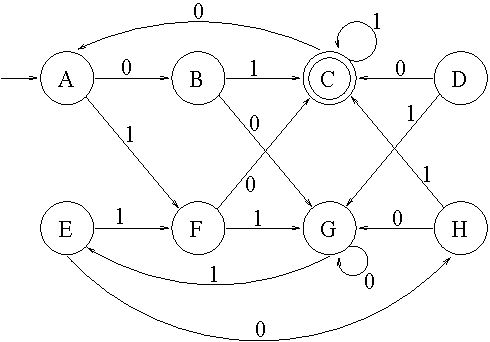
\includegraphics[width=5cm]{figures/7.pdf}
\end{minipage}
\begin{minipage}{5cm}
\begin{tabular}{|c|ccccccc}\hline
  & A & B & C & D & E & F & G \\\hline
B & x &   &   &   &   &   &   \\
C & x & x &   &   &   &   &   \\
D & x & x & x &   &   &   &   \\
E &   & x & x & x &   &   &   \\
F & x & x & x &   & x &   &   \\
G & x & x & x & x & x & x &   \\
H & x &   & x & x & x & x & x
\end{tabular}
\end{minipage}

Distinguishable states are marked by ``x''; the table is only filled
below the diagonal (above is symmetric).
\end{frame}

\begin{frame}

{\bf Theorem:} If two states are not distinguished by the algorithm, then
the two states are equivalent.

{\bf Proof:} Use the Least Number Principle (LPN): any set of natural
numbers has a least element.

Let $\{p,q\}$ be a distinguishable pair, for which the algorithm left
the corresponding square empty, and furthermore, of all such ``bad''
pairs $\{p,q\}$ has a shortest distinguishing string $w$.

Let $w=a_1a_2\ldots a_n$,
$\hat\delta(p,w)$ is accepting \&\ $\hat\delta(q,w)$ isn't.

$w\neq\varepsilon$, as then $p,q$ would be found out in the Basis Case
of the algorithm.

Let $r=\delta(p,a_1)$ and $s=\delta(q,a_1)$.  Then, $\{r,s\}$ are
distinguished by $w'=a_2a_3\ldots a_n$, and since $|w'|<|w|$, they
were found out by the algorithm.

But then $\{p,q\}$ would have been found in the next stage.
\end{frame}

\begin{frame}

{\bf Equivalence of DFAs}

Suppose $D_1,D_2$ are two DFAs.  To see if they are equivalent, i.e.,
$L(D_1)=L(D_2)$, run the table-filling algorithm on their ``union'',
and check if $q^{D_1}_0$ and $q^{D_2}_0$ are equivalent.

Complexity of the Table Filling Algorithm: there are
$n(n-1)/2$ pairs of states.  In one round we check all the pairs of
states to check if their successor pairs have been found
distinguishable; so a round takes $O(n^2)$ many steps.  If in a round
no ``x'' is added, the procedure ends, so there can be no more than
$O(n^2)$ rounds, so the total running time is $O(n^4)$.
\end{frame}

\begin{frame}

{\bf Minimization of DFAs}

Note that the equivalence of states is an equivalence relation.  We
can use this fact to minimize DFAs.

For a given DFA, we run the Table Filling Algorithm, to find all the
equivalent states, and hence all the equivalence classes.  We call
each equivalence class a {\em block}.

In our last example, the blocks would be:
$$
\{E,A\},\{H,B\},\{C\},\{F,D\},\{G\}
$$
The states within each block are equivalent, and the blocks are
disjoint.

We now build a minimal DFA with states given by the blocks as follows:
$\gamma(S,a)=T$, where $\delta(p,a)\in T$ for $p\in S$.
\end{frame}

\begin{frame}
We must show that $\gamma$ is well defined; suppose we choose a
different $q\in S$.  Is it still true that $\delta(q,a)\in T$?

Suppose not, i.e., $\delta(q,a)\in T'$, so $\delta(p,a)=t\in T$, and
$\delta(q,a)=t'\in T'$.  Since $T\neq T'$, $\{t,t'\}$ is a
distinguishable pair.  But then so is $\{p,q\}$, which contradicts
that they are both in $S$.

Theorem: We obtain a minimal DFA from the procedure.

Proof:  Consider a DFA $A$ on which we run the above procedure to
obtain $M$.  Suppose that there exists an $N$ such that
$L(N)=L(M)=L(A)$, and $N$ has fewer states than $M$.

Run the Table Filling Algorithm on $M,N$ together (renaming the
states, so they don't have states in common).  Since $L(M)=L(N)$ their
initial states are indistinguishable.  Thus, each state in $M$ is
indistinguishable from at least one state in $N$.  But then, two
states of $M$ are indistinguishable from the same state of $N\ldots$
\end{frame}

\section{CFGs}

\begin{frame}
\begin{center}
\addtocounter{part}{1}
{\bf Part \Roman{part} \\ Context-free languages}
\end{center}
\end{frame}

\begin{frame}
A \df{context-free grammar (CFG)} is $G=(V,T,P,S)$
--- Variables, Terminals, Productions, Start variable

Ex. $P\longrightarrow\varepsilon|0|1|0P0|1P1$.

Ex. $G=(\{E,I\},T,P,E)$ where $T=\{+,*,(,),a,b,0,1\}$ and $P$ is the
following set of productions:
\begin{align*}
E & \longrightarrow I|E+E|E*E|(E) \\
I & \longrightarrow a|b|Ia|Ib|I0|I1
\end{align*}
If $\alpha A\beta\in(V\cup T)^*$, $A\in V$, and
$A\longrightarrow\gamma$ is a production, then $\alpha
A\beta\Rightarrow\alpha\gamma\beta$.  We use
$\stackrel{*}{\Rightarrow}$ to denote 0 or more steps.

$L(G)=\{w\in T^*|S\stackrel{*}{\Rightarrow}w\}$
\end{frame}

\begin{frame}

{\bf Lemma:}
$L((\{P\},\{0,1\},\{P\longrightarrow\varepsilon|0|1|0P0|1P1\},P))$ is
the set of palindromes over $\{0,1\}$.

{\bf Proof:} Suppose $w$ is a palindrome; show by induction on $|w|$
that $P\stackrel{*}{\Rightarrow}w$.

BS: $|w|\le 1$, so $w=\varepsilon,0,1$, so use
$P\longrightarrow\varepsilon,0,1$.  \\
IS: For $|w|\ge 2$, $w=0x0,1x1$, and
by IH $P\stackrel{*}{\Rightarrow}x$.

Suppose that $P\stackrel{*}{\Rightarrow}w$; show by induction on the
number of steps in the derivation that $w=w^R$.

BS: Derivation has 1 step. \\ 
IS: $P\Rightarrow 0P0\stackrel{*}{\Rightarrow}0x0=w$ (or with 1 instead of 0).
\end{frame}

\begin{frame}

If $S\stackrel{*}{\Rightarrow}\alpha$, then $\alpha\in (V\cup T)^*$,
and $\alpha$ is called a \df{sentential form}.  
$L(G)$ is the set of those
sentential forms which are in $T^*$.

Given $G=(V,T,P,S)$, the \df{parse tree} for $(G,w)$ is a tree with
$S$ at the root, the symbols of $w$ are the leaves (left to right),
and each interior node is of the form:
\begin{center}
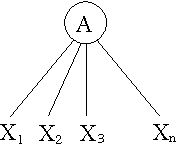
\includegraphics{figures/8.pdf}
\end{center}
whenever we have a rule $A\longrightarrow X_1X_2X_3\ldots X_n$
\end{frame}

\begin{frame}
Derivation: head $\longrightarrow$ body \\
Recursive Inference: body $\longrightarrow$ head

The following five are all equivalent:
\begin{enumerate}
\item  Recursive Inference
\item  Derivation
\item  Left-most derivation
\item  Right-most derivation
\item  Yield of a parse tree.
\end{enumerate}
\end{frame}

\begin{frame}

{\bf Ambiguity of Grammars}

$E\Rightarrow E+E\Rightarrow E+E*E$ \\
$E\Rightarrow E*E\Rightarrow E+E*E$

Two different parse trees!  Different meaning.

A grammar is ambiguous if there exists a string $w$ with two different
parse trees.
\end{frame}

\begin{frame}

A \df{Pushdown Automaton (PDA)} is an $\varepsilon$-NFA with a stack.

Two (equivalent) versions: (i) accept by final state, (ii) accept by
empty stack.

PDAs describe CFLs.

The PDA pushes and pops symbols on the stack; the stack is assumed to
be as big as necessary.

Ex.  What is a simple PDA for $\{ww^R|w\in\{0,1\}^*\}$ ?
\end{frame}

\begin{frame}
Formal definition of a PDA:

$P=(Q,\Sigma,\Gamma,\delta,q_0,Z_0,F)$

$Q$ finite set of states

$\Sigma$ finite input alphabet

$\Gamma$ finite stack alphabet, $\Sigma\subseteq\Gamma$

$\delta(q,a,X)=\{(p_1,\gamma_1),\ldots,(p_n,\gamma_n)\}$

if $\gamma=\varepsilon$, then the stack is popped, if $\gamma=X$, then
the stack is unchanged, if $\gamma=YZ$ then $X$ is replaced $Z$, and
$Y$ is pushed onto the stack

$q_0$ initial state

$Z_0$ start symbol

$F$ accepting states
\end{frame}

\begin{frame}

A \df{configuration} is a tuple $(q,w,\gamma)$:
state, remaining input, contents of the stack

If $(p,\alpha)\in\delta(q,a,X)$, then
$(q,aw,X\beta)\ra(p,w,\alpha\beta)$

{\bf Theorem:} If $(q,x,\alpha)\ra^*(p,y,\beta)$, then
$(q,xw,\alpha\gamma)\ra^*(p,yw,\beta\gamma)$

Acceptance by final state:
$L(P)=\{w|(q_0,w,Z_0)\ra^*(q,\varepsilon,\alpha),q\in F\}$

Acceptance by empty stack:
$L(P)=\{w|(q_0,w,Z_0)\ra^*(q,\varepsilon,\varepsilon)\}$

{\bf Theorem:} $L$ is accepted by PDA by final state iff it is
accepted by PDA by empty stack.

{\bf Proof:} When $Z_0$ is popped, enter an accepting state.  For the
other direction, when an accepting state is entered, pop all the
stack.
\end{frame}

\begin{frame}

{\bf Theorem:} CFGs and PDAs are equivalent.

{\bf Proof:} From Grammar to PDA:
A left sentential form is $\underbrace{x}_{\in T^*}
\overbrace{A\alpha}^{\text{tail}}$

The tail appears on the stack, and $x$ is the prefix of the input that
has been consumed so far.

Total input is $w=xy$, and hopefully
$A\alpha\stackrel{*}{\Rightarrow}y$.

Suppose PDA is in $(q,y,A\alpha)$.  It guesses
$A\longrightarrow\beta$, and enters $(q,y,\beta\gamma)$.

The initial segment of $\beta$, if it has any terminal symbols, they
are compared against the input and removed, until the first variable
of $\beta$ is exposed on top of the stack.

Accept by empty stack.
\end{frame}

\begin{frame}
Ex.  Consider $P\longrightarrow \varepsilon|0|1|0P0|1P1$

The PDA has transitions: \\
$\delta(q_0,\varepsilon,Z_0)=\{(q,PZ_0)\}$ \\
$\delta(q,\varepsilon,P)=\{(q,0P0),(q,0),(q,\varepsilon),(q,1P1),(q,1)\}$\\
$\delta(q,0,0)=\delta(q,1,1)=\{(q,\varepsilon)\}$ \\
$\delta(q,0,1)=\delta(q,1,0)=\emptyset$ \\
$\delta(q,\varepsilon,Z_0)=(q,\varepsilon)$

Consider:
$P\Rightarrow 1P1
\Rightarrow 10P01
\Rightarrow 100P001
\Rightarrow 100001$

\bigskip

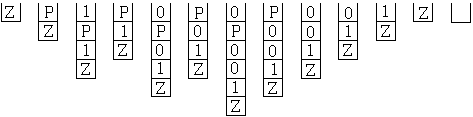
\includegraphics{figures/9.pdf}
\end{frame}

\begin{frame}
From PDA to grammar:

Idea: ``net popping'' of one symbol of the stack, while consuming some
input.

Variables: $A_{[pXq]}$, for $p,q\in Q$, $X\in\Gamma$.  

$A_{[pXq]}\stackrel{*}{\Rightarrow}w$ iff $w$ takes PDA from state $p$
to state $q$, and pops $X$ off the stack.

Productions: for all $p$, $S\longrightarrow A_{[q_0Z_0p]}$, and
whenever we have:
$$
(r,Y_1Y_2\ldots Y_k)\in\delta(q,a,X)
$$ 
$A_{[qXr_k]}\longrightarrow aA_{[rY_1r_1]}A_{[r_1Y_2r_2]}\ldots
A_{[r_{k-1}Y_kr_k]}$ \\
where $a\in\Sigma\cup\{\varepsilon\}$, $r_1,r_2,\ldots,r_k\in Q$ are
all possible lists of states.

If $(r,\varepsilon)\in\delta(q,a,X)$, then we have
$A_{[qXr]}\longrightarrow a$.

{\bf Claim:} $A_{[qXp]}\stackrel{*}{\Rightarrow} w \iff
(q,w,X)\ra^*(p,\varepsilon,\varepsilon)$.
\end{frame}

\begin{frame}
A PDA is deterministic if $|\delta(q,a,X)|\le 1$, and the second
condition is that if for some $a\in\Sigma$ $|\delta(q,a,X)|=1$, then
$|\delta(q,\varepsilon,X)|=0$.

{\bf Theorem:} If $L$ is regular, then $L=L(P)$ for some deterministic
PDA $P$.

{\bf Proof:} ignore the stack.

DPDAs that accept by final state are {\bf not} equivalent to DPDAs
that accept by empty stack.
\end{frame}

\begin{frame}
$L$ has the \df{prefix property} if there exists a pair $(x,y)$,
$x,y\in L$, such that $y=xz$ for some $z$.

Ex. $\{0\}^*$ has the prefix property.

{\bf Theorem:}  $L$ is accepted by a DPDA by empty stack $\iff$ $L$ is
accepted by a DPDA by final state {\bf and} $L$ does not have the
prefix property.

{\bf Theorem:}  If $L$ is accepted by a DPDA, then $L$ is unambiguous.
\end{frame}

\begin{frame}
Eliminating useless symbols from CFG:

$X\in V\cup T$ is \df{useful} if there exists a derivation such that
$S\stackrel{*}{\Rightarrow}\alpha X\beta\stackrel{*}{\Rightarrow}w\in
T^*$ 

$X$ is \df{generating} if $X\stackrel{*}{\Rightarrow}w\in T^*$

$X$ is \df{reachable} if there exists a derivation
$S\stackrel{*}{\Rightarrow}\alpha X\beta$

A symbol is useful if it is generating and reachable.

Generating symbols:
Every symbol in $T$ is generating, and if $A\longrightarrow\alpha$ is
a production, and every symbol in $\alpha$ is generating (or
$\alpha=\varepsilon$) then $A$ is also generating.

Reachable symbols:
$S$ is reachable, and if $A$ is reachable, and
$A\longrightarrow\alpha$ is a production, then every symbol in
$\alpha$ is reachable.
\end{frame}

\begin{frame}
If $L$ has a CFG, then $L-\{\varepsilon\}$ has a CFG without
productions of the form $A\longrightarrow\varepsilon$

A variable is \df{nullable} if
$A\stackrel{*}{\Rightarrow}\varepsilon$

To compute nullable variables: if $A\longrightarrow\varepsilon$ is a
production, then $A$ is nullable, if $B\longrightarrow C_1C_2\ldots
C_k$ is a production and all the $C_i$'s are nullable, then so is $B$.

Once we have all the nullable variables, we eliminate
$\varepsilon$-productions as follows: eliminate all
$A\longrightarrow\varepsilon$.

If $A\longrightarrow X_1X_2\ldots X_k$ is a production, and $m\le k$
of the $X_i$'s are nullable, then add the $2^m$ versions of the rule
the the nullable variables present/absent (if $m=k$, do not add the
case where they are {\em all} absent).
\end{frame}

\begin{frame}
Eliminating unit productions:
$A\longrightarrow B$ \\
If $A\stackrel{*}{\Rightarrow}B$, then $(A,B)$ is a unit pair.

Find all unit pairs: $(A,A)$ is a unit pair, and if $(A,B)$ is a unit
pair, and $B\longrightarrow C$ is a production, then $(A,C)$ is a unit
pair.

To eliminate unit productions: compute all unit pairs, and if $(A,B)$
is a unit pair and $B\longrightarrow\alpha$ is a non-unit production,
add the production $A\longrightarrow\alpha$.  Throw out
all the unit productions.

A CFG is in \df{Chomsky Normal Form} if all the rules are of the form
$A\longrightarrow BC$ and $A\longrightarrow a$.

{\bf Theorem:}  Every CFL without $\varepsilon$ has a CFG in CNF.

{\bf Proof:} Eliminate $\varepsilon$-productions, unit
productions, useless symbols.  Arrange all bodies of
length $\ge 2$ to consist of only variables (by introducing new
variables), and finally break bodies of length $\ge 3$ into a cascade
of productions, each with a body of length exactly 2.
\end{frame}

\begin{frame}

{\bf Pumping Lemma for CFLs:} There exists a $p$ so that any $s$,
$|s|\geq p$, can be written as $s=uvxyz$, and:
\begin{enumerate}
\item  $uv^ixy^iz$ is in the language, for all $i\geq 0$,
\item  $|vy|>0$,
\item  $|vxy|\le p$
\end{enumerate}

Proof:
\begin{center}
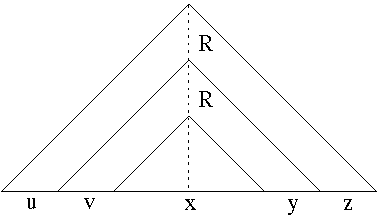
\includegraphics{figures/10.pdf}
\end{center}
\end{frame}

\begin{frame}
Ex. The lang $\{0^n1^n2^n|n\ge 1\}$ is not CF.

So CFL are not closed under intersection:
$L_1=\{0^n1^n2^i|n,i\ge 1\}$ and 
$L_2=\{0^i1^n2^n|n,i\ge 1\}$ are CF, but $L_1\cap L_2=\{0^n1^n2^n|n\ge
1\}$ is not.

{\bf Theorem:} If $L$ is a CFL, and $R$ is a regular language, then
$L\cap R$ is a CFL.

\end{frame}

\begin{frame}[fragile]

%Solution to 5.1.1c in Sipser
$L=\{ww:w\in\{0,1\}^*\}$ is not CF, but $L^c$ is CF.  So CFLs are not
close under complementation either.

We design a CFG for $L^c$.  First note that no odd strings are of the
form $ww$, so the first rule should be:
\begin{align*}
& S\longrightarrow O|E \\
& O\longrightarrow a|b|aaO|abO|baO|bbO
\end{align*}
here $O$ generates all the odd strings.  

$E$ generates
even length strings not of the form $ww$, i.e., all strings of the
form:
\begin{verbatim}
X=|_____0__|_____1__|  or  Y=|_____1__|_____0__|
\end{verbatim}
\end{frame}

\begin{frame}
We need the rule:
$$
E\longrightarrow X|Y
$$
and now
$$
\begin{array}{ll}
X\longrightarrow PQ   &  Y\longrightarrow VW  \\
P\longrightarrow RPR  &  V\longrightarrow SVS \\
P\longrightarrow a    &  V\longrightarrow b   \\
Q\longrightarrow RQR  &  W\longrightarrow SWS \\
Q\longrightarrow b    &  W\longrightarrow a   \\
R\longrightarrow a|b  &  S\longrightarrow a|b
\end{array}
$$

Ex.
\begin{align*}
X &\Ra PQ\Ra RPRQ\Ra RRPRRQ\Ra RRRPRRRQ\Ra RRRRPRRRRQ \\
  &\Ra RRRRRPRRRRRQ \Ra RRRRRaRRRRRQ\Ra RRRRRaRRRRRRQR \\
  &\Ra RRRRRaRRRRRRRQRR \Ra RRRRRaRRRRRRRbRR
\end{align*}
and now the R's can be replaced at will by a's and b's.
\end{frame}

\begin{frame}
CFL are closed under substitution: for every $a\in\Sigma$ we choose
$L_a$, which we call $s(a)$.  For any $w\in\Sigma^*$, $s(w)$ is the
language of $x_1x_2\ldots x_n$, $x_i\in s(a_i)$.

{\bf Theorem:} If $L$ is a CFL, and $s(a)$ is a CFL $\forall
a\in\Sigma$, then $s(L)=\cup_{w\in L}s(w)$ is also CF.

{\bf Proof:}
\begin{center}
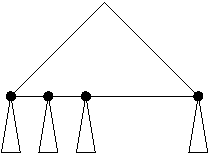
\includegraphics[width=3cm]{figures/11.pdf}
\end{center}

CFL are closed under union, concatenation, $*$ and $+$, homomorphism
(just define $s(a)=\{h(a)\}$, so $h(L)=s(L)$), and reversal (just
replace each $A\longrightarrow\alpha$ by $A\longrightarrow\alpha^R$).
\end{frame}

\begin{frame}
We can test for emptiness: just check whether $S$ is generating.
Test for membership: use CNF of the CYK algorithm (more efficient).

However, there are many {\bf undecidable} properties of CFL:
\begin{enumerate}
\item  Is a given CFG $G$ ambiguous?
\item  Is a given CFL inherently ambiguous?
\item  Is the intersection of two CFL empty?
\item  Given $G_1,G_2$, is $L(G_1)=L(G_2)$?
\item  Is a given CFL everything?
\end{enumerate}
\end{frame}

\begin{frame}
CYK\footnote{Cocke-Kasami-Younger} alg: 
Given $G$ in CNF, and $w=a_1a_2\ldots a_n$,
build an $n\times n$ table.
$w\in L(G)$ if $S\in (1,n)$.  ($X\in(i,j)\iff
X\stackrel{*}{\Rightarrow}a_ia_{i+1}\ldots a_j$.)

Let $V=\{X_1,X_2,\ldots,X_m\}$.  Initialize $T$ as follows:
\begin{tabular}{ll}
for & $(i=1; i\le n; i++)$ \\
    & for $(j=1; j\le m; j++)$
       Put $X_j$ in $(i,i)$ iff $\exists X_j\longrightarrow a_i$
\end{tabular}
Then, for $i<j$:
\begin{tabular}{ll}
for & $(k=i; k<j; k++)$ \\
    & if $(\exists\quad X_p\in (i,k)$ \&\ $X_q\in (k+1,j)$ 
       \&\ $X_r\longrightarrow X_pX_q)$ \\
    & Put $X_r$ in $(i,j)$
\end{tabular}
\footnotesize{%
\begin{tabular}[t]{|p{7mm}|p{7mm}|p{7mm}|p{7mm}|p{7mm}|}\hline
&&&& \\\hline
x&\textcolor{red}{(2,2)}&\textcolor{green}{(2,3)}
&\textcolor{blue}{(2,4)}&{\bf (2,5)} \\\hline
x&x&&&\textcolor{red}{(3,5)} \\\hline
x&x&x&&\textcolor{green}{(4,5)} \\\hline
x&x&x&x&\textcolor{blue}{(5,5)} \\\hline
\end{tabular}}
\end{frame}

\begin{frame}
\df{Context-sensitive grammars (CSG)} have rules of the form:
$$
\alpha\ra\beta
$$
where $\alpha,\beta\in(T\cup V)^*$ and $|\alpha|\le|\beta|$.  A
language is \df{context sensitive} if it has a CSG.

{\bf Fact:}  It turns out that $\text{CSL}=\text{NTIME}(n)$

A \df{rewriting system} (also called a \df{Semi-Thue system}) is a
grammar where there are no restrictions; $\alpha\ra\beta$ for
arbitrary $\alpha,\beta\in(V\cup T)^*$.  

{\bf Fact:}  It turns out that a rewriting system corresponds to the
most general model of computation; i.e., a language has a rewriting
system iff it is ``computable.''

Enter Turing machines $\ldots$
\end{frame}

\begin{frame}

{\bf Chomsky-Schutzenberger Theorem:} If $L$ is a CFL, then there
exists a regular language $R$, an $n$, and a homomorphism $h$, such
that $L=h(\text{PAREN}_n\cap R)$. 

{\bf Parikh's Theorem:} If $\Sigma=\{a_1,a_2,\ldots,a_n\}$, the
signature of a string $x\in\Sigma^*$ is $(\texttt{\#}a_1(x),
\texttt{\#}a_2(x),\ldots,\texttt{\#}a_n(x))$, i.e., the number of
ocurrences of each symbol, in a fixed order.  The signature of a
language is defined by extension; regular and CFLs have the same
signatures.
\end{frame}

\begin{frame}
\begin{minipage}{1.5cm}

\includegraphics[width=1.5cm]{figures/kozen.jpg}
\end{minipage}
\begin{minipage}{6cm}
Automata and Computability \\
Dexter Kozen
\end{minipage}

\begin{minipage}{1.5cm}

\includegraphics[width=1.5cm]{figures/sipser.jpg}
\end{minipage}
\begin{minipage}{6cm}
Intro to the theory of Computation \\
Third edition \\
Michael Sipser
\end{minipage}

\begin{minipage}{1.5cm}
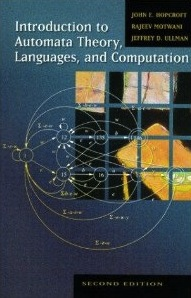
\includegraphics[width=1.5cm]{figures/hopcroft.jpg}
\end{minipage}
\begin{minipage}{9cm}
Intro to automata theory, languages and computation \\
Second edition \\
John Hopcroft, Rajeev Motwani, Jeffrey Ullman \\
{\em There is now a 3rd edition!}
\end{minipage}
\end{frame}

\section{TMs}

\begin{frame}
\begin{center}
\addtocounter{part}{1}
{\bf Part \Roman{part} \\ Turing machines}
\end{center}
\end{frame}

\begin{frame}
Finite control and an infinite tape.

Initially the input is placed on the tape, the head of the tape is
reading the first symbol of the input, and the state is $q_0$.

The other squares contain blanks.

Formally, a \df{Turing machine} is a tuple 
$(Q,\Sigma,\Gamma,\delta)$

where $Q$ is a finite set of \df{states} (always
including the three special states $q_{\text{init}}$,
$q_{\text{accept}}$ and
$q_{\text{reject}}$)

$\Sigma$ is a finite \df{input alphabet} 

$\Gamma$ is a finite \df{tape
alphabet}, and it is always the case that $\Sigma\subseteq\Gamma$ (it
is convenient to have symbols on the tape which are never part of the
input),
$$
\delta:Q\times\Gamma\rightarrow
Q\times\Gamma\times\{\text{Left},\text{Right}\}
$$ 
is the \df{transition function}
\end{frame}

\begin{frame}
\begin{minipage}{5cm}
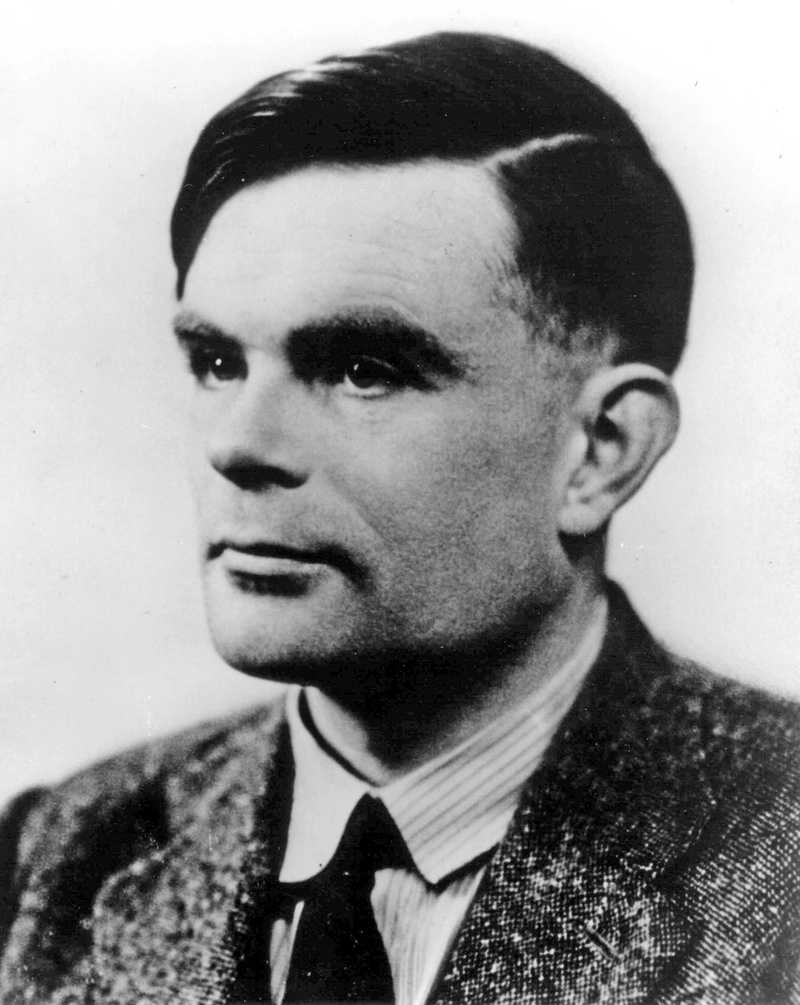
\includegraphics[width=4cm]{figures/AlanTuring.jpg}
\end{minipage}
\begin{minipage}{5cm}
\myhref{http://en.wikipedia.org/wiki/Alan_Turing}{Alan Turing} \\
\end{minipage}
\end{frame}

\begin{frame}
A \df{configuration} is a tuple $(q,w,u)$ where
$q\in Q$ is a state, and where $w,u\in\Gamma^*$, the cursor is on the
last symbol of $w$, and $u$ is the string to the right of $w$.  

A configuration $(q,w,u)$ \df{yields} 
$(q',w',u')$ in one step, denoted as
$(q,w,u)\stackrel{M}{\rightarrow}(q',w',u')$ if one step of $M$ on
$(q,w,u)$ results in $(q',w',u')$.  

Analogously, we
define $\stackrel{M^k}{\rightarrow}$, yields in $k$ steps, and
$\stackrel{M^*}{\rightarrow}$, yields in any number of steps,
including zero steps.  

The initial configuration, $C_{\text{init}}$,
is $(q_{\text{init}},\triangleright,x)$ where $q_{\text{init}}$ is the
initial state, $x$ is the input, and $\triangleright$ is the left-most
tape symbol, which is always there to indicate the left-end of the
tape.
\end{frame}

\begin{frame}
Given a string $w$ as input, we ``turn on'' the TM in the initial
configuration $C_{\text{init}}$, and the machine moves from
configuration to configuration.  

The computation ends when either the
state $q_{\text{accept}}$ is entered, in which case we say that the TM
{\em accepts} $w$, or the state $q_{\text{reject}}$ is entered, in
which case we say that the TM {\em rejects} $w$.  It is possible for
the TM to never enter $q_{\text{accept}}$ or $q_{\text{reject}}$, in
which case the computation does not halt.

Given a TM $M$ we define $L(M)$ to be the set of strings accepted by
$M$, i.e., $L(M)=\{x|\text{$M$ accepts $x$}\}$, or, put another way,
$L(M)$ is the set of precisely those strings $x$ for which
$(q_{\text{init}},\triangleright,x)$ yields an accepting
configuration.
\end{frame}

\begin{frame}
Alan Turing showed the existence of a so called \df{Universal
Turing machine} (UTM); a UTM
is capable of simulating any TM from its description.

A UTM is what we mean by a \df{computer}, capable of running
any algorithm.  The proof is not
difficult, but it requires care in defining a consistent way of
presenting TMs and inputs.

Every Computer Scientist should at some point write a UTM in their
favorite programming language $\ldots$

This exercise really means: designing your own programming language
(how you present descriptions of TMs); designing your own compiler
(how your machine interprets those ``descriptions''); etc.
\end{frame}

\begin{frame}
\df{NTM}

$N$ s.t. $L(N)=\{w\in\{0,1\}^*|\text{ last
symbol of $w$ is 1 }\}$.

\begin{minipage}{5cm}
\begin{align*}
\delta(q_0,0) &=\{(q_0,0,\rightarrow),(q,0,\rightarrow)\} \\
\delta(q_0,1) &=\{(q_0,1,\rightarrow),(r,1,\rightarrow)\} \\
\delta(r,\square) &=\{(\qaccept,\square,\rightarrow)\} \\
\delta(r,0/1) &=\{(q,0,\rightarrow)\}
\end{align*}
\end{minipage}
\begin{minipage}{4cm}
\begin{center}
\Tree [.$q_0011$ [.$0q_011$ [.$01q_01$ [.$011q_0$ $\times$ ] 
[.$011r$ $011\square \qaccept$  ] ] 
[.$01r1$ [.$010q$ $\times$ ] ] ] [.$0q11$ $\times$ ] ] 
\end{center}
\end{minipage}
\end{frame}

\begin{frame}
Different variants of TMs are equivalent (\df{robustness}):
tape infinite in only one direction, or
several tapes.

TM $=$ NTM:
$D$ maintains a sequence of config's on tape 1:
$$
\begin{array}{c|c|c|c|c}\hline
\cdots & \text{config}_1 & \text{config}_2 & \text{config}_3^* & \cdots \\\hline
\end{array}
$$
and uses a second tape for scratch work.

The marked config (*) is the current config.  $D$ copies it to the second
tape, and examines it to see if it is accepting.  If it is, it accepts.

If it is not, and $N$ has $k$ possible moves, $D$ copies the $k$ new
config's resulting from these moves at the end of tape 1, and marks the
next config as current. 

If max nr of choices of $N$ is $m$, and $N$ makes $n$ moves, $D$
examines $1+m+m^2+m^3+\cdots+m^n\approx nm^n$ many configs.
\end{frame}

\begin{frame}

{\bf Undecidability}

We can encode every Turing machine with a string over $\{0,1\}$.  For
example, if $M$ is a TM:
$$
(\{q_1,q_2\},\{0,1\},\delta,\ldots)
$$
and $\delta(q_1,1)=(q_2,0,\rightarrow)$ is one of the transitions,
then it could be encoded as:
$$
\underbrace{0}_{q_1}1
\underbrace{00}_11
\underbrace{00}_{q_2}1
\underbrace{0}_01
\underbrace{0}_\rightarrow11
\underbrace{\ldots\ldots\ldots\ldots\ldots\ldots}_{
\text{\begin{minipage}{3cm}encoding of other\\[-3mm]transitions\end{minipage}}}
$$

Not every string is going to be a valid encoding of a TM (for example
the string 1 does not encode anything in our convention).  

Let all ``bad strings'' encode a default TM $M_{\text{default}}$ which
has one state, and halts immediately, so
$L(M_{\text{default}})=\emptyset$.
\end{frame}

\begin{frame}

\begin{quote}
{\em The intuitive notion of algorithm is captured by the formal
definition of a TM.}
\end{quote}

$$
\ATM=\{\langle M,w\rangle:\text{$M$ is a TM and $M$ accepts
$w$}\},
$$
called the {\em universal language}
\end{frame}

\begin{frame}

{\bf Theorem 6.63:} $\ATM$ is undecidable.


Suppose that it is decidable, and that $H$ decides it.  Then,
$L(H)=\ATM$, and $H$ always halts (observe that $L(H)=L(U)$, but $U$,
as we already mentioned, is not guaranteed to be a decider).  Define a
new machine $D$ (here $D$ stands for ``diagonal,'' since this argument
follows Cantor's ``diagonal argument''):
$$
D(\langle M\rangle):=
\begin{cases}
\text{accept} & \text{if $H(\langle M,\langle M\rangle\rangle)=$ reject} \\
\text{reject} & \text{if $H(\langle M,\langle M\rangle\rangle)=$ accept}
\end{cases}
$$
that is, $D$ does the ``opposite.''  Then we can see that $D(\langle
D\rangle)$ accepts iff it rejects.  Contradiction; so $\ATM$ cannot be
decidable.

\end{frame}

\begin{frame}
It turns out that all nontrivial properties of RE languages are
undecidable, in the sense that the language consisting of codes of TMs
having this property is not recursive.

E.g., the language consisting of codes of TMs whose languages are
empty (i.e., $L_e$) is not recursive.

A \df{property} of RE languages is simply a subset of RE.  A property
is \df{trivial} if it is empty or if it is everything.

If $\mathcal{P}$ is a property of RE languages, the language
$L_{\mathcal{P}}$ is the set of codes for TMs $M_i$ s.t.
$L(M_i)\in\mathcal{P}$.

When we talk about the decidability of $\mathcal{P}$, we formally mean
the decidability of $L_{\mathcal{P}}$.
\end{frame}

\begin{frame}

{\bf Rice's Theorem:} Every nontrivial property of RE languages is
undecidable.

Proof: Suppose $\mathcal{P}$ is nontrivial.  Assume
$\emptyset\not\in\mathcal{P}$ (if it is, consider
$\overline{\mathcal{P}}$ which is also nontrivial).

Since $\mathcal{P}$ is nontrivial, some $L\in\mathcal{P}$,
$L\neq\emptyset$. 

Let $M_L$ be the TM accepting $L$.

For a fixed pair $(M,w)$ consider the TM $M'$: on input $x$, it first
simulates $M(w)$, and if it accepts, it simulates $M_L(x)$, and if
that accepts, $M'$ accepts.

$\therefore$ $L(M')=\emptyset\not\in\mathcal{P}$ if $M$ does not
accept $w$, and $L(M')=L\in\mathcal{P}$ if $M$ accepts $w$.

Thus, $L(M')\in\mathcal{P}\iff(M,w)\in \ATM$, $\therefore$
$\mathcal{P}$ is undecidable.
\end{frame}

\begin{frame}

{\bf Post's Correspondence Problem (PCP)}

An instance of \df{PCP} consists of two finite lists of strings over
some alphabet $\Sigma$.  The two lists must be of equal length:

$A=w_1,w_2,\ldots,w_k$ \\
$B=x_1,x_2,\ldots,x_k$

For each $i$, the pair $(w_i,x_i)$ is said to be a \df{corresponding
pair}.  We say that this instance of PCP has a solution if there is a
sequence of one or more indices:
$$
i_1,i_2,\ldots,i_m\qquad m\geq 1
$$
such that:
$$
w_{i_1}w_{i_2}\ldots w_{i_m}=x_{i_1}x_{i_2}\ldots x_{i_m}
$$
{\bf The PCP is:} given $(A,B)$, tell whether there is a solution.
\end{frame}

\begin{frame}
\begin{minipage}{5cm}
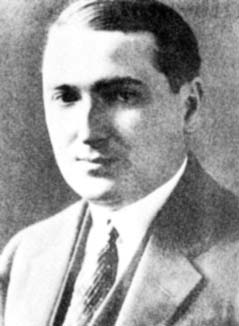
\includegraphics[width=4cm]{figures/EmilLeonPost.jpg}
\end{minipage}
\begin{minipage}{5cm}
\myhref{http://en.wikipedia.org/wiki/Emil_Leon_Post}{Emil Leon Post} \\
\end{minipage}
\end{frame}

\begin{frame}

{\bf Aside:}  To express {\bf PCP} as a language, we let
$L_{\text{PCP}}$ be the language:
$$
\{\langle A,B\rangle|\text{$(A,B)$ instance of PCP with solution}\}
$$

{\bf Example:}  Consider $(A,B)$ given by:

$A=1,10111,10$ \\
$B=111,10,0$

Then $2,1,1,3$ is a solution as:
$$
\underbrace{10111}_{w_2}
\underbrace{1}_{w_1}
\underbrace{1}_{w_1}
\underbrace{10}_{w_3}=
\underbrace{10}_{x_2}
\underbrace{111}_{x_1}
\underbrace{111}_{x_1}
\underbrace{0}_{x_3}
$$
Note that $2,1,1,3,2,1,1,3$ is another solution.  

On the other hand, you can check that:
$A=10,011,101$ \&\
$B=101,11,011$
Does not have a solution.
\end{frame}

\begin{frame}
The {\bf MPCP} has an additional requirement that the first pair in
the solution must be the first pair of $(A,B)$.

So $i_1,i_2,\ldots,i_m$, $m\ge 0$, is a solution to the $(A,B)$
instance of {\bf MPCP} if:
$$
w_1w_{i_1}w_{i_2}\ldots w_{i_m}=x_1x_{i_1}x_{i_2}\ldots x_{i_m}
$$

We say that $i_1,i_2,\ldots,i_r$ is a \df{partial solution} of PCP if
one of the following is the prefix of the other:
$$
w_{i_1}w_{i_2}\ldots w_{i_r}\qquad x_{i_1}x_{i_2}\ldots x_{i_r}
$$
Same def holds for MPCP, but $w_1,x_1$ must be at the beginning.
\end{frame}

\begin{frame}
We now show:

\begin{enumerate}
\item  If {\bf PCP} is decidable, then so is {\bf MPCP}.
\item  If {\bf MPCP} is decidable, then so is $\ATM$.
\item  Since $\ATM$ is {\em not} decidable, neither is {\bf (M)PCP}.
\end{enumerate}
\end{frame}

\begin{frame}
\begin{center}
\fbox{{\bf PCP} decidable $\Longrightarrow$ {\bf MPCP} decidable}
\end{center}

We show that given an instance $(A,B)$ of MPCP, we
can construct an instance $(A',B')$ of PCP such that:
\begin{center}
$(A,B)$ has solution $\iff$ $(A',B')$ has solution
\end{center}

Let $(A,B)$ be an instance of MPCP over the alphabet $\Sigma$.  Then
$(A',B')$ is an instance of PCP over the alphabet
$\Sigma'=\Sigma\cup\{*,\$\}$.

If $A=w_1,w_2,w_3,\ldots,w_k$, then 
$A'=*\textbf{w}_1*,\textbf{w}_1*,\textbf{w}_2*,\textbf{w}_3*,
\ldots,\textbf{w}_k*,\$$.

If $B=x_1,x_2,x_3,\ldots,x_k$, then
$B'=*\textbf{x}_1,*\textbf{x}_1,*\textbf{x}_2,*\textbf{x}_3,
\ldots,*\textbf{x}_k,*\$$.

where if $x=a_1a_2a_3\ldots a_n\in\Sigma^*$, then
$\textbf{x}=a_1*a_2*a_3*\ldots*a_n$.
\end{frame}

\begin{frame}

{\bf For example:} If $(A,B)$ is an instance if MPCP given as:

$A=1,10111,10$ \\
$B=111,10,0$

Then $(A',B')$ is an instance of PCP given as follows:

$A'=*1*,1*,1*0*1*1*1*,1*0*,\$$ \\
$B'=*1*1*1,*1*1*1,*1*0,*0,*\$$
\end{frame}

\begin{frame}
\begin{center}
\fbox{{\bf MPCP} decidable $\Longrightarrow$ $\ATM$ decidable}
\end{center}

Given a pair $(M,w)$ we construct an instance $(A,B)$ of MPCP such
that: 

TM $M$ accepts $w$ $\iff$ $(A,B)$ has a solution.

{\bf Idea:}  The MPCP instance $(A,B)$ simulates, in its partial
solutions, the computation of $M$ on $w$.

That is, partial solutions will be of the form:
$$
\hsh\alpha_1\hsh\alpha_2\hsh\alpha_3\hsh\ldots
$$
where $\alpha_1$ is the initial config of $M$ on $w$, and for all $i$,
$\alpha_i\ra\alpha_{i+1}$.

The string from the $B$ list will always be one config ahead of the $A$
list; the $A$ list will be allowed to ``catch-up'' only when $M$
accepts $w$.
\end{frame}

\begin{frame}
To simplify things,
we may assume that our TM $M$:
\begin{enumerate}
\item  Never prints a blank.
\item  Never moves left from its initial head position.
\end{enumerate}

The configs of $M$ will always be of the form $\alpha q\beta$, where
$\alpha,\beta$ are non-blank tape symbols and $q$ is a state.
\end{frame}

\begin{frame}
Let $M$ be a TM and $w\in\Sigma^*$.  We
construct an instance $(A,B)$ of MPCP as follows:
\begin{enumerate}
\item 
$A$: \hsh  \\
$B$: $\hsh q_0w\hsh$ 

\item 
$A$: $X_1,X_2,\ldots,X_n,\hsh$ \\
$B$: $X_1,X_2,\ldots,X_n,\hsh$ \\
where the $X_i$ are all the tape symbols.

\item To simulate a move of $M$, for all non-accepting $q\in Q$:
\begin{center}
\begin{tabular}{lll}
list $A$ & list $B$ & \\
$qX$     & $Yp$     & if $\delta(q,X)=(p,Y,\rightarrow)$ \\
$ZqX$    & $pZY$    & if $\delta(q,X)=(p,Y,\leftarrow)$ \\
$q\hsh$    & $Yp\hsh$   & if $\delta(q,B)=(p,Y,\rightarrow)$ \\
$Zq\hsh$   & $pZY\hsh$  & if $\delta(q,B)=(p,Y,\leftarrow)$
\end{tabular}
\end{center}
\end{enumerate}
\end{frame}

\begin{frame}
\begin{enumerate}
\setcounter{enumi}{3}
\item If the config at the end of $B$ has an accepting state, then we need
to allow $A$ to catch up with $B$.  So we need for all accepting
states $q$, and all symbols $X,Y$:
\begin{center}
\begin{tabular}{ll}
list $A$ & list $B$ \\
$XqY$    & $q$ \\
$Xq$     & $q$ \\
$qY$     & $q$
\end{tabular}
\end{center}
\item Finally, after using 4 and 3 above, we end up with $x\hsh$ and
$x\hsh q\hsh$, where $x$ is a long string.  Thus we need $q\hsh\hsh$ in $A$ and
$\hsh$ in $B$ to complete the catching up.
\end{enumerate}
\end{frame}

\begin{frame}

{\footnotesize Ex.
%$M=(\{q_1,q_2,q_3\},\{0,1\},\{0,1,B\},\delta,q_1,B,\{q_3\})$,
%\begin{tabular}{c|c|c|c}
%      & 0                     & 1                    & B \\\hline
%$q_1$ & $(q_2,1,\rightarrow)$ & $(q_2,0,\leftarrow)$ & $(q_2,1,\leftarrow)$\\
%\hline
%$q_2$ & $(q_3,0,\leftarrow)$ & $(q_1,0,\rightarrow)$ & $(q_2,0,\rightarrow)$\\
%\hline
%$q_3$ & --- & --- & --- \\
%\end{tabular}
$\delta(q_1,0)=(q_2,1,\rightarrow),
\delta(q_1,1)=(q_2,0,\leftarrow),
\delta(q_1,B)=(q_2,1,\leftarrow)$
$\delta(q_2,0)=(q_3,0,\leftarrow),
\delta(q_2,1)=(q_1,0,\rightarrow),
\delta(q_2,B)=(q_2,0,\rightarrow)$

\begin{tabular}{|l|l|l|l|}\hline
Rule & list $A$ & list $B$      & Source \\\hline\hline
1    & $\hsh$     & ${\hsh}q_101{\hsh}$   &        \\\hline
2    & $0$      & $0$           &        \\
     & $1$      & $1$           &        \\
     & ${\hsh}$     & ${\hsh}$          &        \\\hline
3    & $q_10$   & $1q_2$        & $\delta(q_1,0)=(q_2,1,\rightarrow)$ \\
     & $0q_11$  & $q_200$       & $\delta(q_1,1)=(q_2,0,\leftarrow)$ \\
     & $1q_11$  & $q_210$       & $\delta(q_1,1)=(q_2,0,\leftarrow)$\\ 
     & $0q_1${\hsh} & $q_201${\hsh}     & $\delta(q_1,B)=(q_2,1,\leftarrow)$\\
     & $1q_1${\hsh} & $q_211${\hsh}     & $\delta(q_1,B)=(q_2,1,\leftarrow)$\\
     & $0q_20$  & $q_300${\hsh}     & $\delta(q_2,0)=(q_3,0,\leftarrow)$\\
     & $1q_20$  & $q_310${\hsh}     & $\delta(q_2,0)=(q_3,0,\leftarrow)$\\
     & $q_21$   & $0q_1$        & $\delta(q_2,1)=(q_1,0,\rightarrow)$\\
     & $q_2${\hsh}  & $0q_2${\hsh}      & $\delta(q_2,B)=(q_2,0,\rightarrow)$\\\hline
\end{tabular}
\begin{tabular}{|l|l|l|l|}\hline
4    & $0q_30$  & $q_3$         & \\
     & $0q_31$  & $q_3$         & \\
     & $1q_30$  & $q_3$         & \\
     & $1q_31$  & $q_3$         & \\
     & $0q_3$   & $q_3$		& \\
     & $1q_3$   & $q_3$		& \\
     & $q_30$   & $q_3$		& \\
     & $q_31$   & $q_3$		& \\\hline
5    & $q_3{\hsh}{\hsh}$& ${\hsh}$          & \\\hline
\end{tabular}}
\end{frame}

\begin{frame}
The TM $M$ accepts the input $01$ by the sequence of moves:
$$
q_101\ra
1q_21\ra
10q_1\ra
1q_201\ra
q_3101
$$

We examine the sequence of partial solutions that mimics this
computation of $M$ and eventually leads to a solution.  

We must start with the first pair (MPCP):

$A$: {\hsh} \\
$B$: {\hsh}$q_101${\hsh}

The only way to extend this partial solution is with the corresponding
pair $(q_10,1q_2)$, so we obtain:

$A$: {\hsh}$q_10$ \\
$B$: {\hsh}$q_101{\hsh}1q_2$ 
\end{frame}

\begin{frame}

{\footnotesize
Now using copying pairs we obtain:

$A$: {\hsh}$q_101{\hsh}1$ \\
$B$: {\hsh}$q_101{\hsh}1q_21{\hsh}1$ 

Next corresponding pair is $(q_21,0q_1)$:

$A$: {\hsh}$q_101{\hsh}1q_21$ \\
$B$: {\hsh}$q_101{\hsh}1q_21{\hsh}10q_1$ 

Now careful!  We only copy the next two symbols to obtain:

$A$: {\hsh}$q_101{\hsh}1q_21{\hsh}1$ \\
$B$: {\hsh}$q_101{\hsh}1q_21{\hsh}10q_1{\hsh}1$ 

because we need the $0q_1$ as the head now moves left, and use the
next appropriate corresponding pair which is $(0q_1{\hsh},q_201{\hsh})$ and
obtain:

$A$: {\hsh}$q_101{\hsh}1q_21{\hsh}10q_1{\hsh}$ \\
$B$: {\hsh}$q_101{\hsh}1q_21{\hsh}10q_1{\hsh}1q_201{\hsh}$ 
}
\end{frame}

\begin{frame}

{\footnotesize
We can now use another corresponding pair $(1q_20,q_310)$ right away
to obtain:

$A$: {\hsh}$q_101{\hsh}1q_21{\hsh}10q_1{\hsh}1q_20$ \\
$B$: {\hsh}$q_101{\hsh}1q_21{\hsh}10q_1{\hsh}1q_201{\hsh}q_310$ 

and note that we have an accepting state!  We use two copying pairs to
get:

$A$: {\hsh}$q_101{\hsh}1q_21{\hsh}10q_1{\hsh}1q_201{\hsh}$ \\
$B$: {\hsh}$q_101{\hsh}1q_21{\hsh}10q_1{\hsh}1q_201{\hsh}q_3101{\hsh}$ 

and we can now start using the rules in 4.\ to make $A$ catch up with
$B$:

$A$: $\ldots{\hsh}q_31$ \\
$B$: $\ldots{\hsh}q_3101{\hsh}q_3$ 

and we copy three symbols:

$A$: $\ldots{\hsh}q_3101{\hsh}$ \\
$B$: $\ldots{\hsh}q_3101{\hsh}q_301{\hsh}$ 
}
\end{frame}

\begin{frame}
And again catch up a little:

$A$: $\ldots{\hsh}q_3101{\hsh}q_30$ \\
$B$: $\ldots{\hsh}q_3101{\hsh}q_301{\hsh}q_3$ 

Copy two symbols:

$A$: $\ldots{\hsh}q_3101{\hsh}q_301{\hsh}$ \\
$B$: $\ldots{\hsh}q_3101{\hsh}q_301{\hsh}q_31{\hsh}$ 

and catch up:

$A$: $\ldots{\hsh}q_3101{\hsh}q_301{\hsh}q_31$ \\
$B$: $\ldots{\hsh}q_3101{\hsh}q_301{\hsh}q_31{\hsh}q_3$ 

and copy:

$A$: $\ldots{\hsh}q_3101{\hsh}q_301{\hsh}q_31{\hsh}$ \\
$B$: $\ldots{\hsh}q_3101{\hsh}q_301{\hsh}q_31{\hsh}q_3{\hsh}$ 
\end{frame}

\begin{frame}
And now end it all with the corresponding pair $(q_3{\hsh}{\hsh},{\hsh})$ given by
rule 5.\ to get matching strings:

$A$: $\ldots{\hsh}q_3101{\hsh}q_301{\hsh}q_31{\hsh}q_3{\hsh}{\hsh}$ \\
$B$: $\ldots{\hsh}q_3101{\hsh}q_301{\hsh}q_31{\hsh}q_3{\hsh}{\hsh}$ 

{\bf THEREFORE:} we reduced $\ATM$ to the MPCP.  Now, we can solve
$\ATM$ by producing a carefully crafted instance of MPCP $(A,B)$, and
asking if it has a solution.  If yes, then we know that $M$ accepts
$w$.

Since we have already shown that $\ATM$ is undecidable, MPCP must also
be undecidable.  Thus, PCP is undecidable.

{\bf NEXT:} We can now use the fact that PCP is undecidable to show
that a number of questions about CFLs are undecidable.
\end{frame}

\begin{frame}
Let $A=w_1,w_2,\ldots,w_k$, let $G_A$ be the related CFG given by:
$$
A\longrightarrow w_1Aa_1|w_2Aa_2|\cdots|w_kAa_k|w_1a_1|w_2a_2|\cdots|w_ka_k
$$
Let $L_A=L(G_A)$, the language of the list $A$, and
$a_1,a_2,\ldots,a_k$ are distinct index symbols not in alphabet of
$A$.

The terminal strings of $G_A$ are of the form:
$$
w_{i_1}w_{i_2}\ldots w_{i_m}a_{i_m}\ldots a_{i_2}a_{i_1}
$$

Let $G_{AB}$ be a CFG consisting of $G_A,G_B$, with $S\longrightarrow
A|B$.

$\therefore$ $G_{AB}$ is ambiguous $\iff$ the PCP $(A,B)$ has a
solution.

{\bf Theorem:}  It is undecidable whether a CFG is ambiguous.
\end{frame}

\begin{frame}
$\overline{L_A}$ is also a CFL; we show this by giving a PDA $P$.

$\Gamma_P=\Sigma_A\cup\{a_1,a_2,\ldots,a_k\}$.

As long as $P$ sees a symbol in $\Sigma_A$ it stores it on the stack.

As soon as $P$ sees $a_i$, it pops the stack to see if top of string
is $w_i^R$.  (i) if not, then accept no matter what comes next.  (ii)
if yes, there are two subcases:

(iia) if stack is not yet empty, continue.

(iib) if stack is empty, and the input is finished, reject.

If after an $a_i$, $P$ sees a symbol in $\Sigma_A$, it accepts.
\end{frame}

\begin{frame}

{\bf Theorem:} $G_1,G_2$ are CFGs, and $R$ is a reg.\ exp., then the
following are undecidable problems:
\begin{enumerate}
\item  $L(G_1)\cap L(G_2)\stackrel{?}{=}\emptyset$
\item  $L(G_1)\stackrel{?}{=} L(G_2)$
\item  $L(G_1)\stackrel{?}{=} L(R)$
\item  $L(G_1)\stackrel{?}{=} T^*$
\item  $L(G_1)\stackrel{?}{\subseteq} L(G_2)$
\item  $L(R)\stackrel{?}{\subseteq} L(G_2)$
\end{enumerate}
\end{frame}

\begin{frame}
Proofs: 1. Let $L(G_1)=L_A$ and $L(G_2)=L_B$, then $L(G_1)\cap
L(G_2)\neq\emptyset$ iff PCP $(A,B)$ has a solution.

2.  Let $G_1$ be the CFG for $\overline{L_A}\cup\overline{L_B}$ (CFGs
are closed under union).  Let $G_2$ be the CFG for the reg.\ lang.\
$(\Sigma\cup\{a_1,a_2,\ldots,a_k\})^*$.  

Note
$L(G_1)=\overline{L_A}\cup\overline{L_B}=\overline{L_A\cap L_B}=$
everything but solutions to PCP $(A,B)$.

$\therefore$ $L(G_1)=L(G_2)$ iff $(A,B)$ has no solution.

3.  Shown in 2.

4.  Again, shown in 2.

5.  Note that $A=B$ iff $A\subseteq B$ and $B\subseteq A$, so it
follows from 2.

6.  By 3.\ and 5.
\end{frame}

\section{$\lambda$}

\begin{frame}
\begin{center}
\addtocounter{part}{1}
{\bf Part \Roman{part} \\ $\lambda$-calculus \\ (not in textbook)} 
\end{center}
\end{frame}

\begin{frame}

The set $\Lambda$ of \df{$\lambda$-terms} is the smallest set such
that:
\begin{itemize}
\item $x,y,z\ldots\in\Lambda$ (\df{variables} are in $\Lambda$)
\item if $x$ is a variable and $M$ is $\lambda$-term, then so is
$(\lambda x.M)$ (\df{abstraction})
\item if $M,N$ are $\lambda$-terms then so is $(MN)$
(\df{application})
\end{itemize}

$\text{FV}(M)$ is the set of free variables of $M$.  It is defined
recursively as follows: $\text{FV}(x)=\{x\}$, and $\text{FV}(\lambda
x.M)=\text{FV}(M)-\{x\}$ and
$\text{FV}(MN)=\text{FV}(M)\cup\text{FV}(N)$.

Terms without free variables are \df{closed terms} (also called
\df{combinators}), i.e., $M$ is closed iff $\text{FV}(M)=\emptyset$.

$\text{BV}(M)$ is the set of bounded variables of $M$.
$\text{BV}(x)=\emptyset$, $\text{BV}(\lambda
x.M)=\{x\}\cup\text{BV}(M)$ and $\text{BV}(M)\cup\text{BV}(N)$.
\end{frame}

\begin{frame}
Ex. $\lambda z.z$ is closed, and $\text{FV}(z\lambda x.x)=\{z\}$ while
$\text{BV}(z\lambda x.x)=\{x\}$.  On the other hand
$\text{BV}(x\lambda x.x)=\text{BV}(x\lambda x.x)=\{x\}$.

It is important to realize that two formulas are essentially the same
if they only differ in the names of bounded variables, e.g., $\lambda
x.x$ and $\lambda y.y$ represent (in some sense) the same object.  To
make this concept precise, we introduce the notion of
\df{$\alpha$-equality}, denoted $=_\alpha$.

$M\aeq N$ if $M=N=x$

Note that the equalith on the right ($M=N=x$) is {\em syntactic}
equality and $x$ can be any variable.

$M\aeq N$ if $M=M_1M_2$ and $N=N_1N_2$ and $M_1\aeq N_1$ and $M_2\aeq
N_2$.
\end{frame}

\begin{frame}
Also, $M\aeq N$ if $M=\lambda x.M_1$ and $N=\lambda x.N_1$ and
$M_1\aeq N_1$.

Finally, $M\aeq N$ if $M=\lambda x.M_1$ and $N=\lambda y.N_1$ and
there is a {\em new} variable $z$ such that $M_1\{x\mapsto z\}\aeq
N_1\{y\mapsto z\}$.

Here $M\{x\mapsto N\}$ denotes the $\lambda$-term $M$ where every {\em
free} instance of $x$ has been replaced by the $\lambda$-term $N$, in
such a way that no free variable $u$ of $N$ has been ``caught'' in the
scope of some $\lambda u$.  If $z$ is new, it will never be caught.

We shall soon give a formal definition of substitution.

But first: $\aeq$ is an equivalence relation.  

Ex. $\lambda x.x\aeq \lambda y.y$, $\lambda x.\lambda y.xy\aeq \lambda
z_1.\lambda z_2.z_1z_2$ and $(\lambda x.x)z\aeq(\lambda y.y)z$.

Thus, we think of $\lambda$-terms in terms of their equivalence
classes wrt $\aeq$ relation.
\end{frame}

\begin{frame}
We now define the notion of computation: a \df{redex} is a term of the
form $(\lambda x.M)N$.  The idea is to apply the function $\lambda
x.M$ to the argument $N$.  We do this as follows:
$$
(\lambda x.M)N\rab M\{x\mapsto N\}
$$
This is the so called \df{$\beta$-reduction} rule.  We write $M\rab
M'$ to indicate that $M$ reduces to $M'$.

Ex. $(\lambda x.x)y\rab x\{x\mapsto y\}=y$

(again, note that the equality is a syntactic equality)

$(\lambda x.\lambda y.x)(\lambda x.x)u
\rab(\lambda y.\lambda z.z)u
\rab\lambda z.z$

(application associates to the left, i.e., $MNP=(MN)P$)
\end{frame}

\begin{frame}
Ex. $(\lambda x.\lambda y.xy)(\lambda x.x)
\rab\lambda y.(\lambda x.x)y
\rab\lambda y.y$

The symbol $\srab$ means zero or more applications of $\rab$; from
the previous example,
$(\lambda x.\lambda y.xy)(\lambda x.x)\srab\lambda y.y$.

We use the word {\em reduce} but this does not mean that the terms
necessarily get simpler/smaller.

Ex. $(\lambda x.xx)(\lambda xyz.xz(yz))
\rab(\lambda xyz.xz(yz))(\lambda xyz.xz(yz))$

(note that $\lambda xyz$ abbreviates $\lambda x.\lambda y.\lambda z$,
and that abstractions associate to the right, i.e., $\lambda xyz.M$ is
$\lambda x.(\lambda y.(\lambda z.M))$)
\end{frame}

\begin{frame}
\begin{align*}
(\lambda x.xx)(\lambda y.yx)z & = ((\lambda x.xx)(\lambda y.yx))z
\tag*{[application left associates]} \\
&\rab ((xx)\{x\mapsto (\lambda y.yx)\})z 
\tag*{[substitution]} \\
&= ((\lambda y.yx)(\lambda y.yx))z \\
&\rab ((yx)\{y\mapsto (\lambda y.yx)\})z
\tag*{[substitution]} \\
&= ((\lambda y.yx)x)z \\
&\rab ((yx)\{y\mapsto x\})z
\tag*{[substitution]} \\
&= (xx)z = xxz
\tag*{[application left associates]}
\end{align*}

\begin{align*}
(\lambda x.(\lambda y.(xy))y)z
&\rab (\lambda x.((xy)\{y\mapsto y\}))z \\
&= (\lambda x.(xy))z \\
&\rab (xy)\{x\mapsto z\}=zy
\end{align*}
\end{frame}

\begin{frame}
\begin{align*}
((\lambda x.xx)(\lambda y.y))(\lambda y.y)
&\rab ((xx)\{x\mapsto (\lambda y.y)\})(\lambda y.y) \\
&=((\lambda y.y)(\lambda y.y))(\lambda y.y) \\
&\rab (y\{y\mapsto(\lambda y.y)\})(\lambda y.y) \\
&=(\lambda y.y)(\lambda y.y) \\
&=(\lambda y.y)
\tag*{[just repeating previous line]}
\end{align*}

\begin{align*}
(((\lambda x.\lambda y(xy))(\lambda y.y))w)
&= (((\lambda x.\lambda v.(xv))(\lambda y.y))w)
\tag*{[use $=_\alpha$ so $y$ not ``caught'' by $\lambda y$]} \\
&\rab ((\lambda v.(xv))\{x\mapsto(\lambda y.y)\})w \\
&= (\lambda v.((\lambda y.y)v))w \\
&\rab (\lambda v.v)w \\
&\rab w
\end{align*}
\end{frame}

\begin{frame}
We now give a precise definition of \df{substitution} $M\{x\mapsto N\}$
by structural induction on $M$.

$x\{x\mapsto N\}N=N$

$y\{x\mapsto N\}=y$

$(PQ)\{x\mapsto N\}=(P\{x\mapsto N\})(Q\{x\mapsto N\})$

$(\lambda x.P)\{x\mapsto N\}=\lambda x.P$

$(\lambda y.P)\{x\mapsto N\}=\lambda y.(P\{x\mapsto N\})$ if
$y\notin\text{FV}(N)$ or $x\notin\text{FV}(P)$

$(\lambda y.P)\{x\mapsto N\}=(\lambda z.P\{y\mapsto z\})\{x\mapsto
N\}$ otherwise and $z$ is a new variable
\end{frame}

\begin{frame}
Ex.
\begin{align*}
(\lambda z.yz)\{y\mapsto z\} 
&\aeq (\lambda x.(yz)\{z\mapsto x\})\{y\mapsto z\} \\
&\aeq (\lambda x.((y\{z\mapsto x\})(z\{z\mapsto x\})))\{y\mapsto z\} \\
&\aeq (\lambda x.(yx))\{y\mapsto z\} \\
&\aeq \lambda x.(yx)\{y\mapsto z\} \\
&\aeq \lambda x.((y\{y\mapsto z\})(x\{y\mapsto z\})) \\
&\aeq \lambda x.(zy)
\end{align*}

{\bf Property:} If $x\in\text{FV}(P)$, then
$$
(M\{x\mapsto N\})\{y\mapsto P\}\aeq
(M\{y\mapsto P\})\{x\mapsto N\{y\mapsto P\}\}
$$
\end{frame}

\begin{frame}
A \df{normal form} is a term that does not contain any redexes.

A term that can be reduced to normal form is called \df{normalizable}.

Ex. $\lambda abc.((\lambda x.a(\lambda y.xy))bc)\rab
\lambda abc.(a(\lambda y.by)c)$ where the last term is in normal form
(bec applications associate to the left)

Some terms are not normalizable, e.g., $(\lambda x.xx)(\lambda x.xx)$.

A term $M$ is \df{strongly normalizable} (or \df{terminating}) if all
reduction sequences starting from $M$ are finite.

\df{Weak head normal form}: stop reducing when there are no redexe
left, but without reducing under an abstraction.

Ex. $\lambda abc.((\lambda x.a(\lambda xy))bc)$ is in weak head normal
form.
\end{frame}

\begin{frame}

{\bf FACT:} Our reduction relation $\rab$ is \df{confluent} because
whenever $M\rab M_1$ and $M\rab M_2$, then there exists a term $M_3$
such that $M_1\rab M_3$ and $M_2\rab M_3$.

{\bf Corollary:} Each $\lambda$-term has at most one normal form.

{\bf Proof:} Suppose that a term $M$ has more than one normal form;
i.e., $M\rightarrow^*_\beta M_1$ and $M\rightarrow^*_\beta M_2$, where
$M_1$ and $M_2$ are in normal form.  Then they should both be
reducible to a common $M_3$ (by confluence), but if they are in normal
form that cannot be done.  Contradiction---hence there can be at most
one normal form.

\end{frame}

\begin{frame}

\df{Church's numerals}:

\begin{align*}
\bar{0} &= \lambda x.\lambda y.y \\
\bar{1} &= \lambda x.\lambda y.xy \\
\bar{2} &= \lambda x.\lambda y.x(xy) \\
\bar{3} &= \lambda x.\lambda y.x(x(xy)) \\
        &\vdots \\
\bar{n} &= \lambda x.\lambda y.\underbrace{x(x(x\ldots(x}_{n}y)\ldots)) \\
        &\vdots
\end{align*}
\end{frame}

\begin{frame}
\begin{minipage}{5cm}
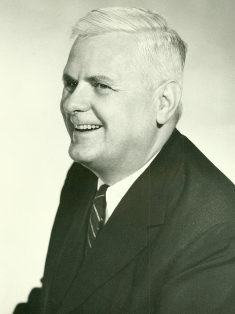
\includegraphics[width=4cm]{figures/AlonzoChurch.jpg}
\end{minipage}
\begin{minipage}{5cm}
\myhref{http://en.wikipedia.org/wiki/Alonzo_Church}{Alonzo Church} \\
\end{minipage}
\end{frame}

\begin{frame}
Consider $S:=\lambda xyz.y(xyz)$
\begin{align*}
S\bar{n} &= S(\lambda xy\underbrace{x(x(x\ldots(x}_{n}y)\ldots))) \\
&\rab \lambda yz.y(\lambda xy.\underbrace{x(x(x\ldots(x}_{n}y)\ldots))yz) \\
&\aeq \lambda yz.y(\lambda xw.\underbrace{x(x(x\ldots(x}_{n}w)\ldots))yz) \\
&\rab \lambda yz.y(\lambda w.\underbrace{y(y(y\ldots(y}_{n}w)\ldots))z) \\
&\rab \lambda yz.\overbrace{y(\underbrace{y(y(y\ldots(y}_{n}}^{n+1}z)
\ldots))) \aeq \overline{n+1}
\end{align*}
so $S(\bar{n})=\overline{n+1}$, i.e., $S$ is the successor fn.
\end{frame}

\begin{frame}

Define $\text{ADD}:=\lambda xyab.(xa)(yab)$.

\begin{align*}
\text{ADD}\bar{n}\bar{m}
&\rab (\lambda yab.(\bar{n}a)(yab))\bar{m} \\
&\rab \lambda ab.(\text{\colorbox{yellow}{$\bar{n}a$}})
(\text{\colorbox{orange}{$\bar{m}a$}}b) \\
&\rab \lambda ab.(
\text{\colorbox{yellow}{$\lambda
y\underbrace{a(a(a\ldots(a}_{n}y)\ldots))$}})
[(\text{\colorbox{orange}{$\lambda
y\underbrace{a(a(a\ldots(a}_{m}y)\ldots))$}})b] \\
&\rab \lambda ab.(
\text{\colorbox{yellow}{$\lambda
y\underbrace{a(a(a\ldots(a}_{n}y)\ldots))$}})
[\text{\colorbox{green}{$\underbrace{a(a(a\ldots(a}_{m}b)\ldots))$}}] \\
&\rab \lambda ab.(\underbrace{\underbrace{a(a(\ldots(a}_{n}
\underbrace{(a(a\ldots(a}_{m}}_{n+m}b)\ldots)))\ldots))) \\
&\aeq\overline{n+m}
\end{align*}
\end{frame}

\section{RFs}

\begin{frame}
\begin{center}
\addtocounter{part}{1}
{\bf Part \Roman{part} \\ Recursive Functions \\ (not in textbook)} 
\end{center}
\end{frame}

\begin{frame}

A \df{partial function} is a function
$$
f:(\mathbb{N}\cup\{\infty\})^n\longrightarrow
\mathbb{N}\cup\{\infty\}, \quad n\ge 0
$$
such that $f(c_1,\ldots,c_n)=\infty$ if some $c_i=\infty$.

$\text{Domain}(f)=\{\vec{x}\in\mathbb{N}^n:f(\vec{x})\neq\infty\}$
where $\vec{x}=(x_1,\ldots,x_n)$.

$f$ is \df{total} if $\text{Domain}(f)=\mathbb{N}^n$, i.e., $f$ is
always defined if its arguments are defined.
\end{frame}

\begin{frame}

A \df{Register Machine (RM)} is a computational model specified by a
program $P=\langle c_0,c_1,\ldots,c_{h-1}\rangle$, consisting of a
finite sequence of commands.

The commands operate on registers $R_1,R_2,R_3,\ldots$, each capable
of storing an arbitrary natural number.

\bigskip

\begin{tabular}{l|c|l}
command & abbrev. & parameters \\\hline
$R_i\leftarrow 0$ & $Z_i$ & $i=1,2,\ldots$ \\
$R_i\leftarrow R_i+1$ & $S_i$ & $i=1,2,\ldots$ \\
goto $k$ if $R_i=R_j$ & $J_{ijk}$ & $i,j=1,2,\ldots$ \amp\
$k=0,1,2,\ldots h$
\end{tabular}
\end{frame}

\begin{frame}
An example RM program that copies $R_i$ into $R_j$:

\begin{tabular}{lll}
$c_0$: & $R_j\leftarrow 0$ & $Z_j$ \\
$c_1$: & goto 4 if $R_i=R_j$ & $J_{ij4}$ \\
$c_2$: & $R_j\leftarrow R_j+1$ & $S_j$ \\
$c_3$: & goto 1 if $R_1=R_1$ & $J_{111}$ \\
$c_4$:
\end{tabular}

Formally, the program is $\langle Z_j,J_{ij4},S_j,J_{111}\rangle$.
\end{frame}

\begin{frame}

{\bf Semantics of RM's}

A \df{state} is an $m+1$-tuple
$$
\langle K,R_1,\ldots,R_m\rangle
$$
of natural numbers, where $K$ is the instruction counter (i.e., the
number of the next command to be executed), and $R_1,\ldots,R_m$ are
the current values of the registers ($m$ is the max
register index referred to in the program).

Given a state $s=\langle K,R_1,\ldots,R_m\rangle$ and a program
$P=\langle c_0,c_1,\ldots,c_{h-1}\rangle$, the next state,
$s'=\text{Next}_P(s)$ is the state resulting when command $c_K$ is
applied to the register values given by $s$.

We say that $s$ is a \df{halting state} if $K=h$, and in this case
$s'=s$.
\end{frame}

\begin{frame}
Suppose the state $s=\langle K,R_1,\ldots,R_m\rangle$ and the command
$c_k$ is $S_j$, where $1\le j\le m$.  Then,
$$
\text{Next}_P(s)=\langle
K+1,R_1,\ldots,R_{j-1},R_j+1,R_{j+1},\ldots,R_m\rangle
$$

Ex. Give a formal definition of the function $\text{Next}_P$ for the cases
in which $c_K$ is $Z_i$ and $J_{ijk}$.
\end{frame}

\begin{frame}
A computation of a program $P$ is a finite or infinite sequence
$s_0,s_1,\ldots$ of states such that $s_{i+1}=\text{Next}_P(s_i)$. 

If the sequence is finite, then the last state must be a halting
state, in which case that computation is halting---we say that $P$ is
halting starting in state $s_0$.

A program $P$ computes a (partial) function $f(a_1,\ldots,a_n)$ as
follows.  Initially place $a_1,\ldots,a_n$ in $R_1,\ldots,R_n$ and set
all other registers to 0.  Start execution with $c_0$, i.e., the
initial state is
$$
s_0=\langle 0,a_1,\ldots,a_n,0,\ldots,0\rangle
$$
If $P$ halts in $s_0$, the final value of $R_1$ must be
$f(a_1,\ldots,a_n)$ (which then must be defined).  If $P$ fails to
halt, then $f(a_1,\ldots,a_n)=\infty$.
\end{frame}

\begin{frame}
We say $f$ is \df{RM-computable} (or just \df{computable}) if $f$ is
computed by some RM program.

{\bf Church's Thesis:}  Every algorithmically computable function is
RM computable.

Ex. Show $P=\langle J_{234},S_1,S_3,J_{110}\rangle$ computes $f(x,y)=x+y$.

Ex. Write RM programs that compute $f_1(x)=x\stackrel{.}{-}1$ and
$f_2(x,y)=x\cdot y$.  Be sure to respect the input/output conventions
for RMs.
\end{frame}

\begin{frame}
$f$ is defined from $g$ and $h$ by \df{primitive recursion (pr)} if
\begin{align*}
& f(\vec{x},0)=g(\vec{x}) \\
& f(\vec{x},y+1)=h(\vec{x},y,f(\vec{x},y))
\end{align*}
we allow $n=0$ so $\vec{x}$ could be missing.
The following high-level program computes $f$ from $g,h$ by
pr:
\begin{tabbing}
$u\leftarrow g(\vec{x})$ \\
for \= $z:0\ldots(y-1)$ \\
    \> $u\leftarrow h(\vec{x},z,u)$ \\
end for
\end{tabbing}

$f_+(x,y)=x+y$ can be define by pr as follows:
\begin{align*}
& x+0=x \\
& x+(y+1)=(x+y)+1
\end{align*}
In this case $g(x)=x$ and $h(x,y,z)=z+1$.
\end{frame}

\begin{frame}
$f$ is defined from $g$ and $h_1,\ldots,h_m$ by \df{composition} if
$f(\vec{x})=g(h_1(\vec{x}),\ldots,h_m(\vec{x}))$, where
$f,h_1,\ldots,h_m$ are each $n$-ary and $g$ is $m$-ary.

\df{Initial functions:}
\begin{tabular}{ll}
$Z$ & $0$-ary constant function equal to 0 \\
$S$ & $S(x)=x+1$ \\
$\pi_{n,i}(x_1,\ldots,x_n)=x_i$ & infinite class of \df{projection}
functions
\end{tabular}

$f$ is \df{primitive recursive (pr)} if $f$ can be obtained from the
initial functions by finitely many applications of primitive recursion
and composition.

{\bf Proposition:} Every pr function is total.
\end{frame}

\begin{frame}

{\bf Theorem:} Every pr function is RM-computable.

{\bf Proof:} We show every pr $f$ is computable by a program which
upon halting leaves all registers 0 except $R_1$ (which contains the
output).  We do this by induction on the def of pr fns.

Base case: each initial fn is computable by such an RM program.

$Z$ is just $\langle Z_1\rangle$ \\
$S(x)=x+1$ is $\langle S_1\rangle$ \\
$\pi_{n,i}(x_1,\ldots,x_n)$ depends on whether $i=1$ or $i\neq 1$.  In
the first case the program is $\langle Z_2,\ldots,Z_n\rangle$.  In the
second case it is $\langle
\underbrace{Z_1,J_{i14},S_1,J_{111}}_\text{``Copy $R_i$ to
$R_1$''},Z_2,\ldots,Z_n\rangle$.
\end{frame}

\begin{frame}
Induction step:  
Composition: Assume that $g,h_1,\ldots,h_m$ are computable by programs
$P_g,P_{h_1},\ldots,P_{h_m}$, where these programs leave all registers
zero except $R_1$.

We must show that $f$ is computable by a program $P_f$ where
$f(\vec{x})=g(h_1(\vec{x}),\ldots,h_m(\vec{x}))$.  At the start
$\vec{x}=x_1,\ldots,x_n$ are in registers $R_1,\ldots,R_n$, with all
other registers zero.

Program $P_f$ must proceed (at a high level) as follows: it must move
$\vec{x}$ out of the way, to some high-numbered registers.  Then it
must compute $h_i(\vec{x})$, for each $i$, by moving a $\vec{x}$ to
$R_1,\ldots, R_n$, simulating $P_{h_i}$, and then moving the result
from $R_1$ out of the way.

At the end it must move the value of $h_i(\vec{x})$ to $R_i$, for each
$i$, and simulate $P_g$.

Primitive recursion: implement the high-level program given following
the definition of pr.
\end{frame}

\begin{frame}
Is the converse true?  Is every computable fn pr?

No.  Some computable fns are not total.

Is every total computable fn pr?

No.  We can show this by a diagonal argument: each pr fn can be
encoded as a number; let $f_1,f_2,f_3,\ldots$ be the list of all pr
functions.

We are only interested in unary fns, so if $f_i$ has arity greater
than one, we replace it by $S$ (the unary successor function).  Let
the new list be $g_1,g_2,g_3,\ldots$, where $g_i=f_i$ if $f_i$ was
unary, and $g_i=S$ otherwise.

Let $U(x,y)=g_x(y)$, so $U$ is a total computable fn.  However, $U$ is
not pr; for suppose that it is.  Then so is $D(x)=S(U(x,x))$.  If $U$
were pr, so would be $D$.  

But if $D$ is pr, then $D=g_e$ for some $e$.  This gives us a
contradiction, since $g_e(e)=D(e)=g_e(e)+1$.
\end{frame}

\begin{frame}
We can in fact give a concrete example of a total computable fn, which
is not primitive recursive. 

The \df{Ackermann function} is defined as follows:
$$
A_0(x)=\begin{cases}
x+1 & \text{if $x=0$ or $x=1$} \\
x+2 & \text{otherwise}
\end{cases}
$$
and $A_{n+1}(0)=1$ and $A_{n+1}(x+1)=A_n(A_{n+1}(x))$.

We can prove by induction on $n$ that $A_n(x)$ is total for all $n$,
and therefore so is $A(n,x)=A_n(x)$.  Also, $A$ is computable since it
can be computed with an RM program following the recursion given
above.

Note that $A_2(x)=2^x$ while
$A_3(x)=\left. 2^{2^{2^{\iddots^2}}}\right\}$ of height
$x$.
\end{frame}

\begin{frame}

{\bf Lemma:} For each $n$, $A_n$ is pr.

{\bf Proof:} By induction on $n$; the work is in the base case.

{\bf Fact:}  For every pr fn $h(\vec{x})$, there exists an $n$ so that
for sufficiently large $B$, if $\min\{\vec{x}\}>B$ then
$h(\vec{x})<A_n(\max\{\vec{x}\})$, i.e., $A_n$ dominates $h$.  

Then, if $A(n,x)=A_n(x)$, then $A$ is not pr; in fact, $F(x)=A(x,x)$
is not pr, since $A$ cannot dominate itself.


\end{frame}

\begin{frame}
We let $\mu$ denote the least number operator.  More precisely,
$f(\vec{x})=\mu y[g(\vec{x},y)=0]$ if
\begin{enumerate}
\item  $f(\vec{x})$ is the least number $b$ such that
$g(\vec{x},b)=0$,
\item  $g(\vec{x},y)\neq\infty$ for $i<b$.
\end{enumerate}
$f(\vec{x})=\infty$ if no such $b$ exists.

If $g$ is computable and $f(\vec{x})=\mu y[g(\vec{x},y)=0]$ then $f$
is also computable:

\begin{tabbing}
for \= $y=0\ldots\infty$ \\
    \> if \= $g(\vec{x},y)=0$ then \\
    \>    \> output $y$ and exit \\
    \> end if \\
end for
\end{tabbing}
\end{frame}

\begin{frame}
A function $f$ is \df{recursive} if $f$ can be obtained from the
initial functions by finitely many applications of composition,
primitive recursion, and minimization.

{\bf Theorem:} Every recursive function is computable.

In the 1940s Kleene showed that the converse of the above theorem is
also true: every computable function is recursive.

We next prove this converse: every computable fn is recursive.
\end{frame}

\begin{frame}
First we assign a \df{G{\"o}del number} $\hsh P$ to every program
$P$:

\begin{tabular}{l|c|c|c}
command $c$ & $Z_i$ & $S_i$ & $J_{ijm}$ \\\hline
&&& \\
code    $\hsh c$ & $2^i$ & $3^i$ & $5^i7^j11^m$
\end{tabular}

By the {\bf Fundamental Theorem of Arithmetic} these codes are unique.

Let $p_0<p_1<p_2<\cdots=2<3<5<\cdots$ be the list of all primes, in
order.  Then, if $P=\langle c_0,c_1,\ldots,c_{h-1}\rangle$,
$$
\hsh P=p_0^{\hsh c_0}p_1^{\hsh c_1}\cdots p_{h-1}^{\hsh c_{h-1}}
$$

Encode the state $s$ of a program as follows:
$$
\hsh s=\hsh\langle K,R_1,\ldots,R_m\rangle
=p_0^kp_1^{R_1}\cdots p_m^{R_m}
$$
\end{frame}

\begin{frame}
\begin{minipage}{5cm}
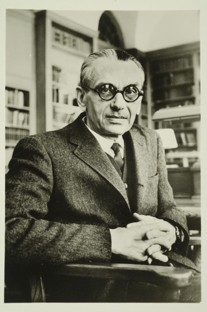
\includegraphics[width=4cm]{figures/KurtGodel.jpg}
\end{minipage}
\begin{minipage}{5cm}
\myhref{http://en.wikipedia.org/wiki/Kurt_Godel}{Kurt G{\"o}del} \\
\end{minipage}
\end{frame}

\begin{frame}
\begin{minipage}{5cm}
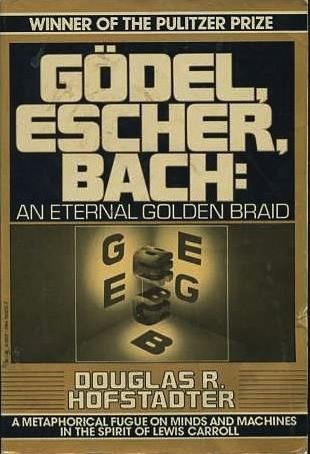
\includegraphics[width=4cm]{figures/geb.jpg}
\end{minipage}
\begin{minipage}{5cm}
G{\"o}del, Escher, Bach \\
\end{minipage}
\end{frame}

\begin{frame}
\begin{minipage}{5cm}
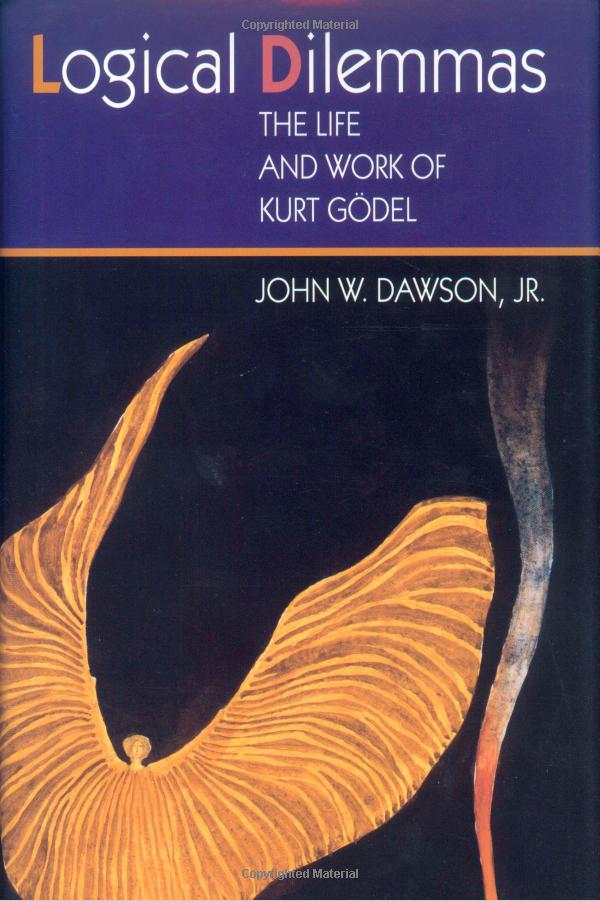
\includegraphics[width=4cm]{figures/logicaldilemmas.png}
\end{minipage}
\begin{minipage}{5cm}
A serious study of G{\"o}del \\
\end{minipage}
\end{frame}

\begin{frame}
\begin{minipage}{5cm}
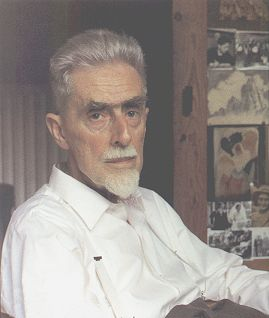
\includegraphics[width=4cm]{figures/escher_photo.jpg}
\end{minipage}
\begin{minipage}{5cm}
\myhref{http://en.wikipedia.org/wiki/M._C._Escher}{Maurits Escher} \\
\end{minipage}
\end{frame}

\begin{frame}
\begin{center}
\begin{minipage}{8cm}
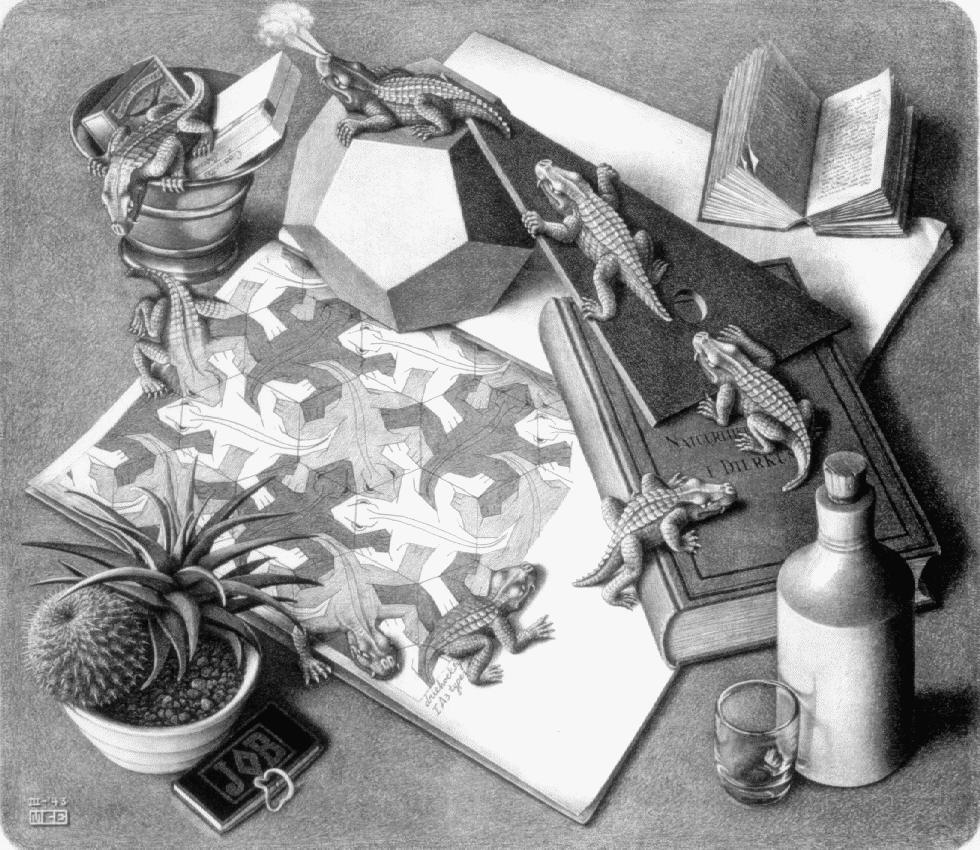
\includegraphics[width=8cm]{figures/escher1.jpg}
\end{minipage}
\end{center}
\end{frame}

\begin{frame}
\begin{center}
\begin{minipage}{6cm}
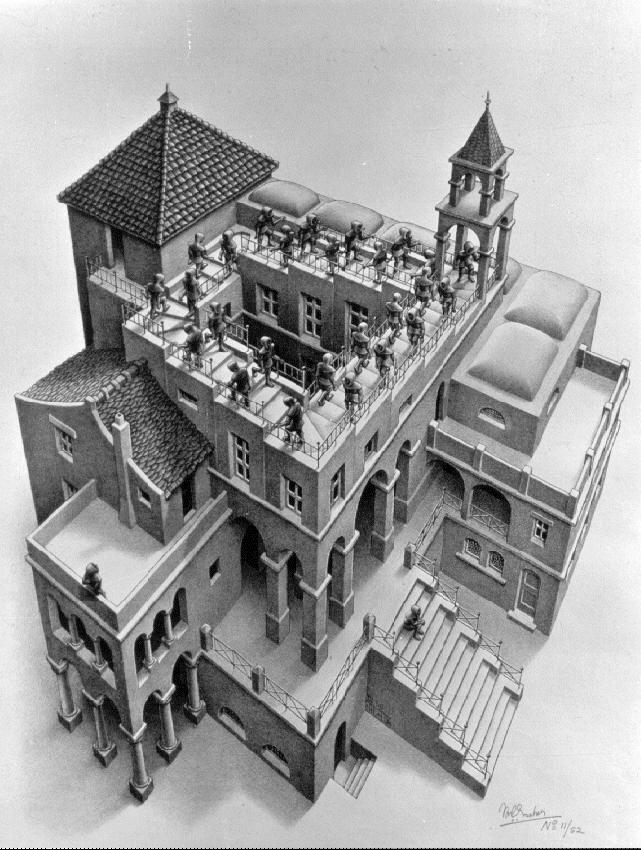
\includegraphics[width=6cm]{figures/escher2.jpg}
\end{minipage}
\end{center}
\end{frame}

\begin{frame}
\begin{center}
\begin{minipage}{6cm}
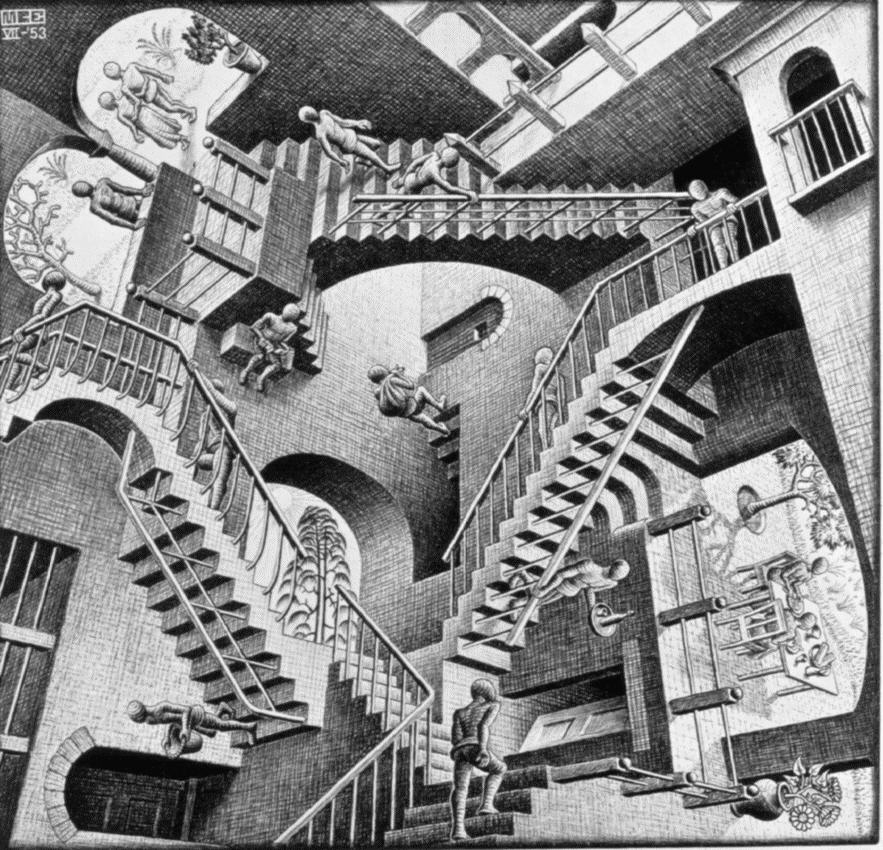
\includegraphics[width=6cm]{figures/escher3.jpg}
\end{minipage}
\end{center}
\end{frame}

\begin{frame}
\begin{center}
\begin{minipage}{6cm}
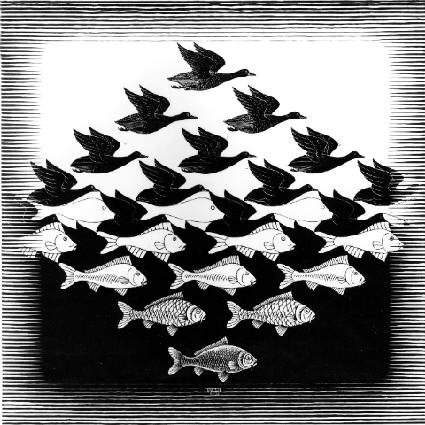
\includegraphics[width=6cm]{figures/escher4.jpg}
\end{minipage}
\end{center}
\end{frame}

\begin{frame}
\begin{center}
\begin{minipage}{8cm}
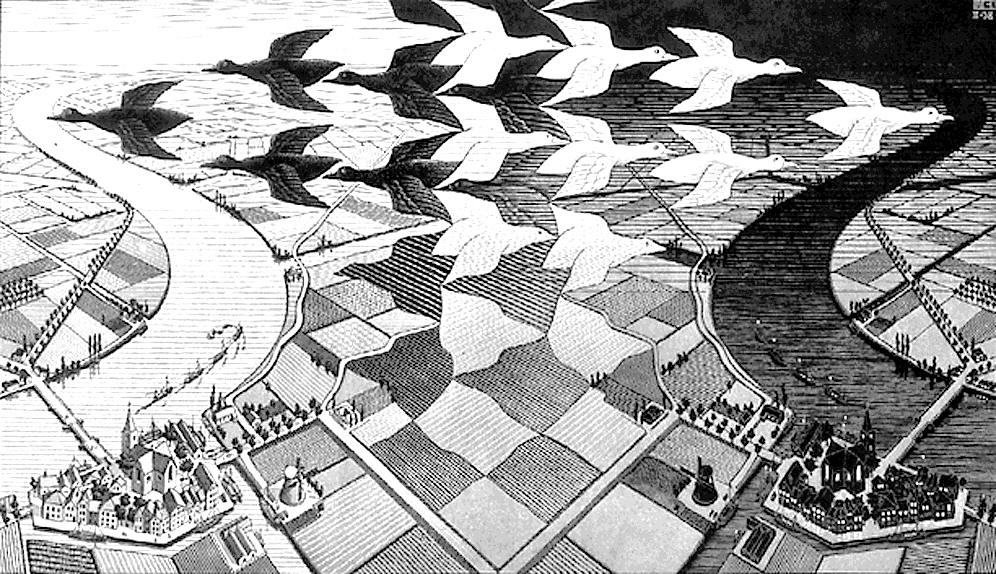
\includegraphics[width=8cm]{figures/escher5.jpg}
\end{minipage}
\end{center}
\end{frame}


\begin{frame}
Ex.  
\begin{align*}
& \hsh S_1=3^1=3 \\
& \hsh \langle S_1\rangle=2^{\hsh S_3}=2^3=8 \\
& \hsh \langle Z_1,S_1,J_{111}\rangle=2^{\hsh Z_1}\cdot
3^{\hsh S_1}\cdot 5^{\hsh J_{111}}=
2^{2^1}\cdot 3^{3^1}\cdot 5^{(5^17^111^1)}=4\cdot 27\cdot 5^{385}
\end{align*}

Distinct programs get distinct codes, and given a code we can extract
the (unique) program encoded by it \\
(or decide that it is not a code
for any program).

Ex. Given the number $10871635968$ we decompose it (uniquely) as a
product of primes:
$$
10871635968
=2^{27}\cdot 3^{4}
=2^{3^3}\cdot 3^{2^2}
=2^{\hsh \textcolor{red}{S_3}}\cdot 3^{\hsh \textcolor{red}{Z_2}}
=\hsh\langle \textcolor{red}{S_3},\textcolor{red}{Z_2}\rangle
$$
\end{frame}

\begin{frame}
We let $\text{Prog}(z)$ be a predicate that is true iff $z$ is the
code of some program $P$.  $\text{Prog}(z)$ is a pr predicate.

%We let $\hat{z}$ be $z$ if $\text{Prog}(z)$ is true, and 1 otherwise.

We let 
$$
\{z\}=\begin{cases}
\text{program $P$ such that $z=\hsh P$} & \text{if $P$ exists} \\
\text{the empty program $\langle\rangle$} & \text{otherwise}
\end{cases}
$$

The function $\text{Nex}(u,z)=u'$ is defined as follows: $u'$ is the
state resulting from a single step of $\{z\}$ on state $u$.  Nex is
pr.
\end{frame}

\begin{frame}
If $u_0,u_1,\ldots,u_t$ is the sequence of codes for the successive
states in a computation, then we code the entire computation by the
number $y=p_0^{u_0}p_1^{u_1}\cdots p_t^{u_t}$.  

\df{Kleene $T$ predicate:} for each $n\ge 1$ we define the $n+2$-ary
relation $T_n$ as follows: $T_n(z,\vec{x},y)$ is true iff $y$ codes
the computation of $\{z\}$ on input $\vec{x}$.  

{\bf Theorem:} For each $n\ge 1$, $T_n$ is pr.

Let $\{z\}_n$ be the $n$-ary fn computed by program $\{z\}$.

\colorbox{yellow}{\bf Kleene Normal Form Theorem:}  
There is a pr fn $U$ such that
$$
\forall n\ge 1,\qquad
\{z\}_n(\vec{x})=U(\mu yT_n(z,\vec{x},y))
$$
($U(y)$ extracts the contents of the first register in the last state
of computation $y$.)  Thus, every computable fn is recursive.
\end{frame}

\begin{frame}
\begin{center}
\addtocounter{part}{1}
{\bf Part \Roman{part} \\ CONCLUSION}
\end{center}
\end{frame}

\begin{frame}

{\bf Church-Turing thesis:} the following models of computation are
all equivalent:

\begin{itemize}
\item  Rewriting systems
\item  Turing machines
\item  $\lambda$-calculus
\item  Recursive functions
\item  Register machines
\item  \textcolor{darkmagenta}{\bf ZFC-computable}
\end{itemize}

Even more evidence that we have captures the notion of compation: ZFC
is the Zarmelo-Fraenkel set theory together with the Axiom of Choice.
All of mathematics can be formalized in ZFC.

A language $L$ is ZFC-computable if there exists a formula
$\alpha(x)$ such that if $w\in L\Rightarrow\text{ZFC}\vdash\alpha(w)$
and if $w\not\in L\Rightarrow\text{ZFC}\vdash\neg\alpha(w)$.
\end{frame}

\end{document}
